\documentclass[10pt, bigheadings]{scrartcl}

\usepackage{ucs}
\usepackage[ngerman]{babel}
\usepackage[T1]{fontenc}
\usepackage[dvips]{graphicx}
\usepackage[dvips]{xcolor}
%\usepackage{colortbl}
\usepackage{a4wide}
\usepackage{tabularx}
\usepackage{graphicx}
\usepackage{amssymb}
\usepackage{floatflt}

% provides font selecting commands 
\usepackage{xunicode} 

% provides unicode character macros 
\usepackage{xltxtra} 

% provides some fixes/extras 
\usepackage{pdfsync}

%\defaultfontfeatures{Scale=MatchLowercase ,Mapping=tex-text} %\setromanfont{Charis SIL} 
%\setsansfont{Gill Sans} 
%\setmonofont{Pragmata}

%\newfontfamily\secfont{Charis SIL}

%\setkomafont{sectioning}{\secfont}

%\input{nomenclature}

\definecolor{gray20}{rgb}{0.93, 0.93, 0.93}




\begin{document}

\begin{titlepage}
\vspace*{2cm}
\begin{center}
\textbf{\huge Untersuchung und Implementierung von Algorithmen
	zur Zerlegung großer Zahlen}\\
\vspace*{0.5cm}
\begin{Large}
\textbf{>>Primfaktorzerlegung<<\\}
\vspace*{3.5cm}
\textbf{Studienarbeit}\\
im Fachbereich Informationstechnik\\
Studiengang Softwaretechnik\\
der\\
Fachhochschule für Technik Esslingen\\
\vspace*{2cm}
\textbf{Zvonko Krnjajic}\\
\vspace*{0.2cm}
723923
\vspace*{3.5cm}
\end{Large}
\end{center}
\begin{Large}
\begin{tabularx}{\textwidth}{ll}
Betreuer: & Prof. Dr. Ing. Reinhardt Schmidt\\
Bearbeitungszeitraum: & 28.03.2005 bis 15.06.2005
\end{tabularx}
\vspace*{1.5cm}
\end{Large}
\begin{center}
\begin{Large}
\textbf{Esslingen,  Juni 2005}
\end{Large}
\end{center}
\end{titlepage}

\thispagestyle{empty}
\begin{abstract}
Die vorliegende Studienarbeit soll einen Überblick über die Algorithmen zur Zerlegung
großer Zahlen geben. Die Sicherheit von asymetrischen Verschlüsselungsverfahren liegt
in der Schwierigkeit begründet, sehr große Zahlen zu faktorisieren. Diese großen
Zahlen sind Produkte zweier Primzahlen $p$ und $q$, $n = p\cdot q$. Man geht davon aus,
dass es schwer ist, aus gegebenem $n$, $p$ und $q$ zu berechnen. Die meissten Verfahren
beruhen auf Erkenntnissen aus Zeiten von Gauß und Euler, d.h. man weiss wie sie
funktionieren, es scheitert also immer an den Laufzeiten der jeweiligen Algorithmen.
Der erste Block wird deshalb aufbauend auf den Erkenntnissen der frühen Zahlentheoriker
ein Überblick geben wieso eine Zahl zerlegt werden kann und ob diese Zerlegung
(Faktorisierung) eindeutig ist.

Faktorisierungsverfahren teilen sich in zwei Gruppen, die mit exponentieller Laufzeit
und die mit subexponentieller Laufzeit. Die ersten Faktorisierungs-Algorithmen sind
Algorithmen mit denen es einfach ist eine Zahl mit kleinen Primfaktoren zu
zerlegen. Sie bilden weiterhin die Grundlage für einfache Primzahltests zur bestimmung
ob eine Zahl eine Primzahl ist. Je größer die Anzahl der Stellen einer Zahl desto
trickreicher bzw. intelligenter muss man vorgehen. Nach einem kurzen Ausflug in
die Zahlentheorie werden Verfahren vorgestellt mit denen es möglich ist Zahlen bis zu
100 Stellen zu faktorisieren, bei entsprechender Laufzeit. Laufzeiten sind das größte
Problem der Algorithmen. Deshalb wird etwas näher drauf eingegangen.

Der letzte Teil zeigt schliesslich die Integration der Faktorisierungs-Algorithmen
in MATLAB.
\end{abstract}
\newpage

\pagestyle{headings}
\tableofcontents
\newpage

\section{Einleitung}
Die Frage, auf welche Arten sich eine gegebene natürliche Zahl $n>1$ als
Summe zweier ganzer Zahlen schreiben lässt, ist sehr einfach zu
beantworten. Es ist $4=3+1=2+2=1+3$ oder allgemein $a=n+(a-n)$, wobei
$n$ beliebig zwischen $1$ und $n-1$ gewählt werden darf. Man bekommt so
ganz systematisch alle möglichen Zerlegungen. Die entsprechende Frage
bezüglich des Produkts lässt sich dagegen nicht so allgemein
entscheiden.

Wichtige Grundbausteine der Kryptographie sind Funktionen, die
leicht berechnet, aber schwer invertiert werden können. Durch sie
kann zum Beispiel verhindert werden, daß ein Angreifer den Schlüssel
berechnen kann, wenn er eine Nachricht und den dazugehörigen Geheimtext
vorliegen hat. In der Kryptologie nutzten Public-Key Verfahren solche
Funktionen zur Verschlüsselung. Faktorisierungsprobleme z.B. werden
speziell in RSA- und Rabin-Kryptosystemen ausgenutzt. Ein weiteres
hartes Problem ist die Berechnung von diskreten Logarithmen
das vom ElGamal-Krytosystem genützt wird.

Das Fehlen von effizienten Algorithmen zur Primfaktorzerlegung einer
ganzen Zahl macht eine Faktorisierung in kurzer Zeit unmöglich.
Für relativ kleine Zahlen ist eine Zerlegung mit der Probedivision
möglich. Die Komplexität wächst jedoch mit der Größe der Zahl. Wird
die zu untersuchende Zahl um ein paar Stellen vergrößert, benötigt
die Probedivision die 100 fache Zeit.

Bisher bekannte Faktorisierungsverfahren
haben zwar ein deutlich besseres Zeitverhalten als die Faktorisierung
mit der Probedivision, doch für die Zerlegung von in
der Kryptologie verwendenten Zahlen mit über 200 Dezimalstellen würden
diese Verfahren Jahre brauchen. Ob es schnellere Verfahren gibt,
ist nicht bekannt, aber auch nicht auszuschließen.

Peter Shor zeigte 1994 einen praktisch verwendbaren Algorithmus für
Quantencomputer. Der in den Forschungslabors von AT\&T arbeitende
Mathematiker konnte beweisen, daß mit dieser neuen Generation von
Rechnern die zur Zeit am häufigsten benutzten Geheimcodes ohne Probleme
zu knacken sind. Eine Umsetzung dieses Algorithmus wäre eine Gefahr für
die bestehende Kryptographie.

\section{Aufgabenstellung}
In dieser Studienarbeit sollen einige aus der Literatur bekannte
Faktorisierungsverfahren untersucht und implementiert werden. Die
Implementation erfolgt in C mit Hilfe der GNU multiple precision
library, kurz GMP. Als weiterer Schritt sollen die
Faktoriserungsverfahren in MATLAB Integriert werden, d.h. ein Aufruf
aus MATLAB soll möglich sein. Die Verfahren dienen dann als Ergänzung
zur bestehenden "crytlib".
Nicht alle Verfahren eignen sich um große Zahlen in entsprechender Zeit
zu faktorisieren deshalb wird jedes Verfahren auf die Laufzeit geprüft.
Zudem muss man unterscheiden ob sich eine Zahl aus kleinen bzw. großen
Primfaktoren zusammensetzt. Vergleiche der Faktorisierungsverfahren
werden aufzeigen welche Verfahren für die jewelige Situation am
günstigsten sind.

\newpage
\section{Primzerlegung}
\subsection{Natürliche, ganze Zahlen}
Das Rechnen mit natürlichen Zahlen geht auf das Zählen zurück. Die Addition
der Zahlen $n$ und $m$ dient der Vorhersage, wie viele Objekte man bekommt,
wenn $n$ Objekte mit $m$ anderen Objekten zusammengebracht werden. Aus
dieser Vorstellung heraus ist dann auch klar das etwa $n + m = m + n$ gilt.
Die Subtraktion natürlicher Zahlen $n$, $m$ lässt sich so erklären, dass
die Aussage $k = n - m$ äquivalent sein soll mit $n = k + m$. Bleiben wir
im Bereich der natürlichen Zahlen so ist offenbar $n-m$ nicht für jedes
Paar $n$, $m$ definiert. Man muss die Menge der natürlichen Zahlen
erweitern zur Menge der ganzen Zahlen. Mit
${\mathbb N}=\{1, 2, 3, 4, ...\}$ wird die Menge der natürlichen Zahlen
bezeichnet. Je nach Vereinbarung ist die $0 \in {\mathbb N}$ bzw.
$0 \in {\mathbb Z}$. Die Menge ${\mathbb N}$ ist eine echte Teilmenge der
Menge ${\mathbb Z}=\{..., -3, -2, -1, 0, 1, 2, 3, 4, ...\}$ aller ganzen
Zahlen. Man sagt auch das die ${\mathbb N}$ Zahlen isomorph in ${\mathbb Z}$
eingebettet sind. Es gibt gute Gründe dafür, die zahlentheoretischen
Untersuchungen sofort in ${\mathbb Z}$ durchzuführen. Zu einem lässt sich in
${\mathbb Z}$ uneingeschränkt subtrahieren und zum anderen ist ${\mathbb Z}$
der richtige Ausgangsbereich für spätere Verallgemeinerungen.

\subsubsection*{Eigenschaften der ganzen Zahlen}
Die ganzen Zahlen bilden einen Ring bezüglich der Addition und der
Multiplikation, d. h. sie können ohne Einschränkung addiert, subtrahiert
und multipliziert werden. Dabei gelten Rechenregeln wie das Kommutativgesetz
und das Assoziativgesetz für Addition und Multiplikation, außerdem gelten
die Distributivgesetze. Die Menge ${\mathbb Z}$ ist bzgl. der Addition
$+$ eine kommutative Gruppe. Statt kommutative Gruppe sagt man auch
abelsche Gruppe.

Eine weiter wichtige Eigenschaft von ${\mathbb Z}$ ist die
Nullteilerfreiheit. Aus $a\cdot b =  0$ mit $a, b \in {\mathbb Z}$
folgt $a = 0$ oder $b = 0$. Aus der Nullteilerfreiheit folgt die
Regel, ein Produkt ist nur dann null, wenn wenigstens
ein Faktor null ist. Daraus ergibit sich die Kürzungsregel aus
$a\cdot b = a\cdot c$ folgt $b = c$.

Die Division ist in ${\mathbb Z}$ eingeschränkt. Die Menge ${\mathbb Z}$
bezüglich der Multiplikation bildet keine abelsche Gruppe. Eine
Gleichung $2\cdot x = 1$ hat keine Lösung in ${\mathbb Z}$, da ${\mathbb Z}$
kein Körper ist. Der kleinste Körper, der ${\mathbb Z}$ enthält, ist
${\mathbb Q}$.

\subsection{Teilbarkeit}
Die Tatsache das ${\mathbb Z}$ kein Körper ist, ist dafür verantwortlich
das es in ${\mathbb Z}$ eine Zahlentheorie gibt. Die Frage, wann
$a \in {\mathbb Z}$ durch $d \in {\mathbb Z}$ teilbar ist, ist die Urfrage
der Zahlentheorie.

Ist $d$ ein Teiler von $a$, so nennt man $d$ auch eine in $a$ aufgehende
Zahl und $a$ ein Vielfaches von $d$. Für den Begriff der Teilbarkeit
benötigt man nur die mulitiplikative, nicht aber die additive Struktur
von ${\mathbb Z}$.

Gibt es zu der natürlichen Zahl $a$ Zahlen $d, v \in {\mathbb Z}$ mit
$a = d\cdot v$ so heißt $a$ durch $d$ teilbar, und $d$ ein Teiler von $a$. Als
Kurzschreibweise wird $d|a$ vereinbart.

Offenbar ist mit $a = d\cdot v$ nicht nur $d$, sondern auch $v$ ein Teiler von
$a$. Genauso leicht sieht man, dass die Zahlen 1 und $a$ immer Teiler von
$a$ sind. Man nennt sie triviale Teiler von $a$. Ein Teiler von $a$ der
kein trivialer Teiler ist, heißt echter Teiler.

Unter Benutzung der Subtraktion kann der Begriff der Teilbarkeit auch als
eine lineare Gleichung aufgefasst werden: $d\cdot x - a = 0$ mit Lösungen in
${\mathbb Z}$. Bei dieser Betrachtungsweise ist der Begriff der Teilbarkeit
nichts anderes als die Theorie der linearen Gleichung in einer unbestimmten
über ${\mathbb Z}$.

\subsection{Primzahlen}
Eine erste Aufgabe der Zahlentheorie besteht darin, eine gegebene natürliche
Zahl $a>1$ als ein Produkt von möglichst vielen Faktoren, die alle größer $1$
und kleiner als $a$ selbst sind, zu schreiben. Der Vorteil solcher
Faktorisierungen für praktische Rechnungen ist die Tatsache das es sich mit
kleinen Zahlen bequemer rechnet als mit großen Zahlen. Nun stößt man immer
wieder auf Zahlen die sich allen Faktorisierungsverfahren widersetzen. Sie
lassen sich nicht als Produkt kleinerer Zahlen darstellen. Diese unzerlegbaren
Zahlen haben einen eigenen Namen, man nennt sie Primzahlen.

Eine natürliche Zahl $p$ heißt Primzahl, wenn $1$ und $p$ die einzigen
positiven Teiler von $p$ sind (triviale Teiler) und $p$ keine echten Teiler
hat. Man nennt Primzahlen häufig auch unzerlegbar.

\subsubsection*{Existenz unendlich vieler Primzahlen}
In den \textit{Elementen} von Euklid (Buch IX) findet sich ein Satz der besagt,
dass es unendlich viele Primzahlen gibt. Bei Euklid kommt das Wort
unendlich nicht vor, er formuliert seinen Satz wie folgt: \textit{Die
Primzahlen sind mehr als jede vorgegebene Menge von Primzahlen}. Für den Beweis
nahm Euklid an, dass es endlich viele Primzahlen $p_1, p_2, p_3 , p_n$ gibt,
und konstruierte aus diesen Primzahlen eine neue Primzahl.
Damit hatte man einen Widerspruch zur Annahme.

Betrachtet wird die Zahl $q = 1 + p_1 \cdot p_2 \cdot ... \cdot p_n $. Man
überlegt sich, dass keine der Zahlen $p_1, p_2, p_3, ... , p_n$ ein Teiler von
$q$ sein kann.
Also ist entweder $q$ selbst eine Primzahl, oder aber es exisitert eine weitere
Primzahl $p_n+1 < q$.

Dieser Beweis ist \textit{konstruktiv}, denn er zeigt außer der Gültigkeit des
Ergebnisses auch einen ganz konkreten Weg auf, wie man aus bekannte Primzahlen
neue Primzahlen gewinnen kann. Geht man z.B. von
$M = \left\lbrace 2, 3, 5, 31 \right\rbrace $ aus und konstruiert daraus
$ m = 2 \cdot 3 \cdot 5 \cdot 31 + 1 = 931$, das ist zwar keine Primzahl aber es
gilt $931 = 7 \cdot 7 \cdot 19$, und man bekommt so zwei neue Primzahlen.

\subsubsection*{Mersenne-Primzahlen}
Zahlen der Form $M_n = 2^n - 1 $ werden, dem französischen Mathematiker Mersenne
zu Ehren, Mersenne-Primzahlen bezeichnet. Mersenne unternahm große
Anstrengungen, solche Primzahlen zu finden, und mit Fermat und Descartes
darüber zu korrespondieren. Es läßt sich zeigen das die Zahl $M_n = 2^n -1 $
höchstens dann eine Mersennesche Primzahl, wenn der Exponent $n$ selbst eine
Primzahl ist. Ist nämlich $n$ ein Produkt $n = v\cdot m$ aus natürlichen Zahlen
$u>1, v>1$,  so hat man die Faktorisierung
\begin{center}
{$2^n -1 = (2^u)^v - 1 = (2^n-1)(1+2^u+(2^u)^2+...+(2^u)^{v-1})$},
\end{center}
in der beide Faktoren rechts $>1$ sind. In diesem Fall ist also auch $M_n$
zerlegbar. Es ist nun keineswegs so, dass jede Primzahl $p$ zu einer
Primzahl $2^n-1$ führt. Schon für $p = 11$ erhält man die zusammengesetze
Zahl $M_{11} = 2^{11} - 1 = 2047 = 23 \cdot 89$. Inzwischen hat man mit Hilfe von
Computern noch weiter sehr große Primzahlen $n>257$ gefunden, die
Mersenne-Primzahlen liefern. 1963 fand man eine Mersenne-Primzahl mit
$n = 11213$ die 23-te Mersennesche Primzahl. Das Postamt in Urbana,
würdigte diesen Fund sogar mit einem Poststempel auf dem die Behauptung:
$2^{11213}-1$ \textit{is prime} stand.

\subsubsection*{Fermat-Primzahlen}
Eine zweite Art von Primzahlen sind die Fermatschen Primzahlen. Diese
Primzahlen haben die Form $2^{2^n} +1 $. Diese stehen in einem engen formalen
Zusammenhang mit Mersennschen Primzahlen und spielen eine große Rolle
in der Theorie der Kreisteilung. Der Name ist zu Ehren des großen
französichen Zahlentheoretikers Pierre de Fermat gewählt. Man kennt
nur fünf Fermatsche Primzahlen, und zwar für $n = 0,1,2,3,4$. Fermat
selbst hat noch vermutet, dass für jedes $n \in {\mathbb N}$ wirklich
eine Primzahl $2^{2^n} +1 $ entsteht. Bereits für $n = 5$ ist
$2^{2^5}+1 = 2^{32}+1 $ durch 641 teilbar.

\subsection{Eindeutigkeit der Primzerlegung}
Es ist bekannt, dass man ganze Zahlen in ihre Primfaktoren zerlegen kann. So ist
$168 = 2 \cdot 2 \cdot 2 \cdot 3  \cdot 7 = 2^3 \cdot 3 \cdot 7$ und
$3300 = 2\cdot2\cdot3\cdot5\cdot5\cdot11=2^2\cdot3\cdot5^2\cdot11$.
In der Praxis würde man so vorgehen, dass man erst den kleinsten Primfaktor
bestimmt, die Zahl durch diesen Faktor dividiert, vom Ergebnis wiederum den
kleinsten Primfaktor bestimmt, dividiert und mit dem Ergebnis entsprechend
weiterarbeitet. Es scheint selbstverständlich, dass eine solche Zerlegung in
Primfaktoren nicht nur für bestimmte, sondern für alle ganze Zahlen möglich
ist. Es ist einfach zu zeigen das eine solche Zerlegung exisitert, aber weniger
einfach zu zeigen, dass diese Zerlegung eindeutig ist. Es existieren einige
Eindeutigkeitsbeweise, ein Beweis geht auf Zermelo zurück der zeigte,
dass zu jeder ganzen Zahl es genau eine bis auf die
Reihenfolge der Faktoren eindeutige Zerlegung in ein Produkt aus Primfaktoren
gibt.
\subsection{Hauptsatz der elementaren Zahlentheorie}
Jede ganze Zahl $a \not= 0$ besitzt genau eine Darstellung
\begin{center}
{$a = \varepsilon {p_1}^{m_1} {p_2}^{m_2} \cdot$...$\cdot
\varepsilon\prod_{\varrho = 1}^r {p_\varrho}^{m_\varrho}$}
\end{center}
mit $\varepsilon=\pm1,\ Primzahlen\ p_1 < p_2 < .. < p_n$ und Exponenten
$m_1 >= 1, ... , m_r >= 1$.

Man nennt die durch den Hauptsatz gegebene Zerlegung von $a$ die
kanonische Primzerlegung von $a$.

\newpage

\section{Faktorisierungs-Algorithmen}
\subsection{Implementierung}
Die Implementierung der Faktorisierung-Algorithmen erfolgt in C. Zur
späteren Integration in MATLAB ist es wichtig das die Programme mit
einem C-Compiler übersetzt werden können. Da mit sehr großen Zahlen
gerechnet wird eine Bibliothek zur Langzahlarithmetik verwendet.

Die GMP (GNU multiple precision) ist frei verfügbar und auf fast allen
Betriesbsystemen lauffähig. Die GNU MP ist eine portable freie Bibliothek,
geschrieben in C, für Langzahlarithmetik auf Ganzen und Rationalen Zahlen.
Ihr Hauptziel ist es eine schnellte Arithmetik zur Verfügung zu stellen,
für alle Anwendungen die eine höhere Genauigkeit benötigen als es die
Datentypen in C unterstützten.
Viele Anwendungen benutzen gerade einige hundert Bits zur Darstellung
von Datentypen. Doch es gibt Anwendungen die auf eine höhre Genauigkeit
angwiesen sind und einige Tausend bzw. Millionen von Bits brauchen. Die
Hauptanwendungen für GMP sind die Kryptographie, Kryptoanalyse,
Algebrasysteme und Numerische Methoden.

\subsection{Probedivision}
Bevor eines der aufwändigeren Faktorisierungsverfahren zur Anwendung
kommt, wird man natürlich die vorgegebene Zahl $n$ daraufhin
untersuchen, ob sie kleine Primteiler hat. Berechnet man nur die
Primteiler unterhalb einer Schranke $B$ spricht man auch von
unvollständiger Probedivision. Die Wahrscheinlichkeit, dass eine
große Zufallszahl $n$ überhaupt keine Primteiler $p\leq B$ besitzt,
kann unter Benützung eines Satzes von Mertens recht gut durch
\begin{center}
$ \prod_{p\leq B} (1- \frac{1}{p})\sim \frac{e^{-\gamma}}{log B} \approx
\frac{0.5615}{log B}$
\end{center}
abgeschätzt werden, wobei hier $p$ alle Primzahlen $p\leq B$ durchläuft und
$\gamma \approx 0.5772$ die Eulersche Konstante bezeichnet. Für z.B. $B=10$
beträgt daher die Wahrscheinlichkeit eines totalen Misserfolgs der
Probedivision etwa bei $4.06\%$.

Es gibt einige Varianten der Probedivision. Die erste und einfachste
ist indem bei der Zahl 2 anfangend der Reihe nach durch alle Primzahlen
$p\geq 2$ durch $N$ teilt und so prüft ob $p$ ein Faktor von $N$ ist.
Hat man so einen Faktor gefunden teilt man $N$ so oft durch $p$, bis
das Ergebnis teilerfremd wird.Wenn das nicht klappt
geht man zur nächsten Primzahl über. Das wird solange wiederholt bis
man bei $\sqrt{N}$ angelangt ist. Die verbleibende Zahl ist dann
ebenfalls eine Primzahl und der letzte Faktor von $N$. Doch wie gewinnt
man alle Primzahlen unterhalb einer Schranke $B$ ?

\subsubsection*{Das Sieb des Eratosthenes}

Das Sieb des Eratosthenes wird dem griechischen Mathematiker Eratosthenes
von Kyrene zugeschrieben. Er war Vorsteher der Bibliothek von Alexandria
und fand Lösungen für ganz unterschiedliche Probleme.

Mit einer Schranke $B=100$ funktioniert das Sieb wie folgt. Man schreibe
bzw. belege Speicherplätze mit einer 1, die repräsentativ für die Zahlen
$2, 3, 4, ... , 100$ stehen. Dann ausgehend von der $2$ streiche man
alle Vielfachen $2n$ der Zahl durch bzw. belege die Speicherplätze mit
der $0$. Die kleinste nun noch nicht betrachtete Zahl ist $3$. Mögliche
Teiler, also Teiler, die ungleich $1$ und ungleich der Zahl selbst sind,
wären kleiner. Weil die Zahl $3$ nicht gestrichen wurde, besitzt sie
keinen solchen Teiler und ist damit eine Primzahl. Andererseits folgt,
dass alle Zahlen $3n$ mit $n\geq2$ keine Primzahlen sind. Das Verfahren
wird fortgesetztt, bis alle Zahlen bis zur gewählten Obergrenze erfasst
worden sind. Jede nicht durchgestrichene Zahl ist dann eine Primzahl.

Die Probedivision läßt sich so implementieren das einmal eine Liste
von Primzahlen, entweder als Bit-Array oder alternativ immer
die Hälfte der Differenz einer Primzahl zur vorhergehenden Primzahl
gespeichert wird. In letzterem Fall benötigt man für jede
Primzahl <1.872.851.947 nur ein Byte Speicherplatz. Alternativ
kann man Bibliotheksfunktionen benützen die Primzahlen liefern.

Die GNU MP besitzt einige Zahlentheoretische Funktionen, unter anderem
auch die Funktion \textit{mpz\_next\_prim\_p(mpz\_t op)} die
Primzahlen $p > op$ liefert.

\subsubsection*{Großer Primzahlsatz}

Es ist offensichtlich das die Verteilung  der Primzahlen immer dünner
wird. Es gibt z.B. 168 Primzahlen zwischen 1 ud 1000, 77 Primzahlen
zwischen 199 000 und 200000  und 49 Primzahlen zwischen $10^9$ und
$10^9+1000$. Die Anzahl der Primzahlen, die kleiner oder gleich n sind
wird mit $\pi(n)$ bezeichnet. Die Primzahlverteilungsfunktion ist eine
Treppenfunktion.  Auf den ersten Blick erscheint es hoffnunglos, genauere
Angaben über die Größenordnung von $\pi(n)$ zu machen.

Dem 15 jährigen Gauss gelang es, durch Studium von numerischen
Primzahltabellen, eine Vergleichsfunktion zu entdecken, die wie die
Funktion $\pi(n)$ wächst und viel einfacher zu handhaben ist als die
Primzahlverteilungsfunktion $\pi(n)$ gibt die Anzahl der Primzahlen im
Intervall $[2,n] $ an.
\begin{center}
Es ist $lim_{k\rightarrow\infty} \frac{\pi(n)ln(n)}{n} = 1$. Damit
ist für große $n \in {\mathbb N}$ der Wert von $\pi(n)$ ungefähr
$\frac{n}{ln(n)}$.
\end{center}
Der Primzahlsatz besagt, dass die Funktion von Gauss $\frac{n}{ln(n)}$
die $\pi(n)$ Funktion so gut approximiert das der Quotient beliebig
dicht bei 1 liegt. Der Beweis wurde allerdings erst 100 Jahre später
von Hadamard und Vallee-Poussin erbracht.

Nach der Rechnung mit der Approximation von Gauss gibt es für große Zahlen
etwa $\pi(n) = \frac{n}{ln(n)}$ Primzahlen. Sollte versucht werden,
eine Zahl mit 150 Stellen, die  aus zwei  etwa gleichgroßen Faktoren
besteht durch Probedivision zu  Faktorisieren, müssten ungefähr
$\frac{10^75}{ln(10^75)}=5,79\cdot10^{72}$ Primzahlen getestet werden.
Es dürfte damit offensichtlich sein, dass die Faktorisierung mit der
Probedivison praktisch nicht durchführbar ist, und für Angriffe auf moderne
Verschlüsselungverfahren unbrauchbar ist.

Im Durchschnitt werden, falls $p$ ein Faktor von $n$ $O(\frac{p}{ln(p)})$ Operationen
gebraucht um einen Teiler zu finden. Im schlimmsten Fall $O(\frac{\sqrt{n}}{ln(n)})$.
Man kann es sich leicht klar machen, wenn man $n$ eine Primzahl ist, man
alle Primzahlen $p<n$ überprüfen müssten. Deshalb wird bei jedem
Faktorisierungsverfahren erst geprüft ob $n$ eine Primzahl ist. So
kann unnötige Rechnung vermieden werden. In jedem Iterationsschritt
hat man eine konstante Anzahl von arithmetischen Operationen mit Zahlen
in der Größenordnung von $n$ die man ungefähr mit $O((log\ n)^2)$
abschätzen kann. Somit wäre der Gesamtaufwand der
Probedivision $O(\frac{p}{ln(p)}(log\ n)^2)$.

Die Probedivision ist für Zahlen geeignet, die aus kleinen Faktoren
besteht. Oft wird die Probedivision dazu verwendet von einer Zahl
herauszufinden ob sie kleine Teiler enthält. Bis zu einer Schranke
z.B. $10^6$, werden dann die Teiler entfernt und mit einem anderem
Verfahren vollständig Faktorisiert.\\\\\\
{\it
\textbf{Beispiel:}\\\\
Es soll die Zahl $n=420$ faktorisiert werden.\\\\
Der erste Schritt besteht aus einem Primzahltest und
testet ob $n$ prim ist. Ist $n$ nicht prim kann die Faktorisierung losgehen:\\\\
1. Schritt: Testen ob die erste Primzahl $2$ ein Teiler von $n$ ist, $420\equiv0\ mod\ 2 \rightarrow$
wir haben ein Teiler gefunden. Die Zahl $n$ wird jetzt so oft wie möglich durch $2$
geteilt bis das Ergebnis teilerfremd zur $2$ ist. Als Ergebnis erhalten wir
$\frac{420}{2} = 210, \frac{210}{2} = 105$.\\\\
2. Schritt: Testen ob die zweite Primzahl $3$ ein Teiler ist, $105\equiv 0\ mod\ 3 \rightarrow$
ein weiterer Teiler. Ergebnis $\frac{105}{3} = 35$.\\\\
3. Schritt: Testen ob die dritte Primzahl $5$ ein Teiler ist, $35\equiv 0\ mod\ 5 \rightarrow$ der
nächste Teiler.\\\\
Als Ergebnis erhalten wir die komplette Faktorisierung von $420 = 2^2\cdot3\cdot5\cdot7$.\\\\
}
Bei der Probedivision ergeben sich zwei Probleme. Bei der Faktorisierung einer
sehr großen Zahl müssen möglicherweise sehr viele Primzahlen ermittelt oder
gespeichert vorliegen. Besteht die Zahl $n$ aus etwa zwei gleichgroßen Primfaktoren
$s,t$ muss im schlimmsten Fall durch alle Primzahlen $p<s$ bzw. $p<t$ geteilt werden.
Wird versucht eine zusammengesetzte Zahl $n$ mit üblichen 150 Stellen mit der
Probedivision zu faktorisieren, sieht man erst nach einer einfachen Rechnung
welche unglaubliche Zeit man dafür brauchen würde.\\\\
{\it
\textbf{Beispiel:}\\\\
Es soll eine aus etwa zwei gleichgroßen Primfaktoren zusammengesetzte Zahl $n$
faktorisiert werden.\\\\
Nach dem großen Primzahlsatz gilt: $\frac{10^{75}}{ln(10^{75})} = 5,79\cdot10^{72}$.
Ein Pentium 4 bei einer Taktfrequenz von 3 GHz kann ungefähr $6\cdot10^9 FLOPS$
erreichen, d.h. wir können ungefähr $10^9$ Zahlen pro Sekunde testen.\\\\
Aus $\frac{5,79\cdot10^{72}}{6\cdot10^9} = 9,65\cdot10^{62}$ und
$\frac{9,65\cdot10^{62}}{60\cdot60\cdot24\cdot365} = 3,13\cdot10^{55}$ folgt das
man ungefähr $\mathbf{10^{55} Jahre}$ brauchen würde um die Zahl $n$ zu faktorisieren!
}

\subsubsection*{Anwendungsbeispiele:}
{\it
Die Tabelle zeigt ein paar Faktorisierungsbeispiele der jeweiligen Verfahren. In weiteren
Kapiteln werden ein Verfahren nach dem anderen aufgelistet und die Stärken und Schwächen
anhand konkreter Beispiele gezeigt. Die Zeit entspricht der kompletten Faktorisierung.
}
\begin{center}
\begin{tabular}{|l|l|l|l|l|}
\hline
Nr. & Verfahren & zu faktorisierende Zahl $n$ & kleinster Primfaktor $p$ & Zeit in s\\
\hline
$1$& Probedivision & $11226205405133$ & $3350527$ & $5$\\
$2$&	& $447327829808987$ & $21150209$ & $35$\\
$3$&	& $40300721895586853$  & $200750663$ & $304$\\
$4$&	& $403007218955868532$ & $2$ & $<1$\\
$5$&	& $403007218955868532112$ & $2$ & $<1$\\
$6$&	& $40300721895586853211212312312$ & $2$ & $<1$\\
\hline
\end{tabular}
\end{center}
{\it
Für kleine Primfaktoren ist die Probedivision unschlagbar wie man sehr
schnell am letzten $n$ erkennt. Sobald aber die Primfaktoren
etwa gleichgroß sind wird die Probedivision sehr sehr langsam.
}
\subsection{Fermat}
Das kleine Teiler einer großen Zahl mit der Probedivision gefunden werden können
ist plausibel und überrascht nicht besonders. Erstaunlich ist es aber das auch
Teiler von $n$ die nahe bei $\sqrt{n}$ liegen und daher als sehr groß eingestuft
werden leicht zu finden sind. Dieses Faktorisierungsverfahren geht auf Fermat zurück.

Seine Idee besteht darin, dass man versucht eine ungerade Zahl $n$ in der Form
$n=u^2 - v^2$ mit natürlichen Zahlen $u$ und $v$ darzustellen. So kann man
trivialerweise die Zahl $n$ als Differenz zweier Quadrate auffassen und man hat
so eine Faktorisierung nach der 3. binomischen Formel in der Form $n=(u+v)(u-v)$
gefunden.

Das wir jede natürliche Zahl als Differenz zweier Quadrate darstellen können
läßt sich einfach zeigen. Aus $n = a\cdot b$ folgt
\begin{center}
$ a = x + y$\\
$ b = x - y$.
\end{center}
Durch Addition und Subtraktion von $a$ und $b$ erhält man
\begin{center}
$ a+b = 2x$\\
$ a-b = 2y$,
\end{center}
auflösen nach $x$ und $y$ liefert
\begin{center}
$ x = \frac{1}{2}(a+b)$\\
$ y = \frac{1}{2}(a-b)$.
\end{center}
Schreibt man jetzt $x$ und $y$ als Differenz zweier Quadrate erkennt man
sofort die Richtigkeit der Annahme.
\begin{center}
$x^2-y^2 = \frac{1}{4}(a+b)^2-(a-b)^2 = \frac{1}{4}(a^2+2ab+b^2-a^2+2ab-b^2) = a\cdot b$
\end{center}

Ausgehend davon das unsere Primfaktoren $p$ und $q$ die gleiche
Stellenzahl haben ist das erste in Frage kommende $u = \lceil n \rceil$.
Ist $u$ ein genaus Quadrat so gilt $v = \sqrt{u^2 - n}$ für den
zweiten Faktor. Ist das nicht der Fall müsste $u$ laufend imkrementiert
werden und jeweils überprüft werden ob $v$ eine Quadratzahl ist.

Der Algorithmus sieht dann folgendermaßen aus. Als ersten Schritt setzt man
$u_1 = \lceil n \rceil$ und $v_1 = {u_1}^2 - n$. Im Falle dass $\sqrt{v_1}$ eine
Quadratzahl ist, haben wir eine nichttriviale Faktorisierung von $n$
gefunden und wir können $n = (u_1 - \sqrt{v_1})(u_1 + \sqrt{v_1})$ schreiben.
Haben wir kein Erfolg, setzen wir $u_2 = u_1 + 1$, $v_2 = {u_2}^2 - n$
und testen wiederum ob $v_2$ eine Quadratzahl ist.

Bei der Berechnugn von $v_n$ können wir noch eine Vereinfachung vornehmen.
Betrachtet man sich die Folge $v_1, v_2 , v_3 , ..., v_n$ kann man erkennen,
dass nachfolgende $v_{n+1}$ durch Addition $v_{n+1} = v_n+2$ ermittelt werden können.\\\\
Aus $u_2 = u_1 + 1$, $v_2 = {u_2}^2 - n$ folgt\\
\begin{center}
\begin{tabular}{ll}
$v_2$ & $= {u_2}^2 - n = (u_1 + 1)^2 - n = {u_1}^2 + 2u_1 + 1 - n$\\
      &	$= {u_1}^2 - n + 2u_1 +1$\\
$\mathbf{v_2}$ & $\mathbf{= v_1 + 2u_1 + 1}$.\\

$v_3$ & $= {u_3}^2 - n = {u_2 +1}^2 = {u_2}^2 + 2u_2 + 1 - n$\\
	& $= {u_2}^2 - n + 2u_2 + 1$\\
	& $= v_2 + 2u_2 +1$\\
$\mathbf{v_3}$	& $\mathbf{= v_2 + 2u_1 +3}$\\
 $\mathbf{v_4}$	& $\mathbf{ = v_3 + 2u_1 + 5}$\\
 $\mathbf{v_5}$	& $\mathbf{ = v_4 + 2u_1 + 7}$ ...\\
\end{tabular}
\end{center}

Man erkennt, dass man nachfolgende Quadratzahlen $v_{n+1}$ durch Addition
von der Zahl $2$ gewinnen kann $v_{n+1} = v_n + 2$. Aus den so gewonnenen Quadratzahlen
wird die Wurzel gezogen und überprüft ob das Ergebnis eine ganze Zahl ist.
Die GMP liefert hier die Funktion \textit{mpz\_perfect\_square\_p(v)} mit der
eine \textit{perfekte} Wurzel geprüft werden kann.

Um den mehrfachen Aufruf von \textit{mpz\_perfect\_square\_p(v)} zu vermeiden,
werden nur die Reste $r = u^2 - y^2 - n$ protokolliert und jeweils $u$ bzw.
$v$ inkrementiert, je nachdem ob $r>0$ oder $r<0$ ist. Für den Fall $r = 0$
haben wir eine Zerlegung $n = x^2 - y^2$.\\\\
{\it
\textbf{Beispiel:}\\\\
Die Zahl $n = 1052507$ soll faktorisiert werden:\\\\
1. Schritt: Man setzt $u_1 = \lceil\sqrt{1052507}\rceil = 1026$.\\
2. Schritt: Berechnen von  $v_1 = {u_1}^2 - n = 1026^2 - 1052507 = 169$.\\
3. Schritt: Überprüfen ob $v_1$ Quadratzahl ist.
	$v_1 = 169$, $\sqrt{169} = 13$, $13$ ist Quadratzahl \\
4. Schritt: Berechnen der Faktoren
$n = (u_1 - \sqrt{v_1})(u_1 + \sqrt{v_1}) = (1026 - 13)(1026 + 13) = 1013\cdot1039$.\\
Als Ergebnis erhält man die Faktorisierung der Zahl $n=1052507=1013\cdot1039$.\\\\
}

Der Worst-Case tritt dann auf wenn die zusammengesetzte Zahl in der From
$n = 3p$ ist. Diese Faktorisierung wird erst für $u = (n+9)/6$ entdeckt.
Im schlechtesten Fall haben also $O(n)$ Operationen. In diesem Fall schneidet
die Fermat-Faktorisierung schlechter ab als die Probedivision.

\subsubsection*{Anwendungsbeispiele:}
{\it
Die Fermat-Faktorisierung ist nur dann effizient wenn $n$ zwei beieinander liegende
Faktoren besitzt. Am Beispiel der Zahlen $7,8,9$ wird es sichtbar. Es wird
auch direkt sichtbar, wie die Zeiten der Zahlen $n$ mit kleinen Faktoren
immer größer werden obwohl der kleinste Primfaktor gleich ist. Umgekehrt
steigen die Zeiten bei der Probedivision bei Primfaktoren,
die in der Gegend von $\sqrt{n}$ liegen }
\begin{center}
\begin{tabular}{|l|l|l|l|l|}
\hline
Nr. & Verfahren & zu faktorisierende Zahl $n$ & kleinster Primfaktor $p$ & Zeit in s\\
\hline
$1$& Probedivision & $11226205405133$ & $3350527$ & $5$\\
$2$&	& $447327829808987$ & $21150209$ & $35$\\
$3$&	& $40300721895586853$  & $200750663$ & $304$\\
$4$&	& $403007218955868532$ & $2$ & $<1$\\
$5$&	& $403007218955868532112$ & $2$ & $<1$\\
$6$&	& $40300721895586853211212312312$ & $2$ & $<1$\\
\hline
$7$& Fermat & $11226205405133$ & $3350527$ & $<1$\\
$8$&	& $447327829808987$ & $21150209$ & $<1$\\
$9$&	& $40300721895586853$  & $200750663$ & $<1$\\
$10$&	& $403007218955868532$ & $2$ & $9$\\
$11$&	& $403007218955868532112$ & $2$ & $>500$\\
$12$&	& $40300721895586853211212312312$ & $2$ & $>500$\\
$13$&	& $614735324543115119$ & $784050413$ & $<1$\\
\hline
\end{tabular}
\end{center}
Die Stärke der beiden Methoden zu vereinigen war eine Idee von Lehman. Er erzielte
so eine Laufzeitverbesserung mit der Kombination beider Verfahren.

Die Lehmann-Methode wendet die Probedivision für $d<n^\frac{1}{3}$ an und geht dann
zur Suche nach Quadratzerlegungen von
$kn = x^2 - y^2$ für verschiedene $k, 1\leq k \leq n^{\frac{1}{3}}$, und $x$ in der
Nähe von $2\sqrt{km}$ über. Für die Lehman-Methode die nicht implementiert wurde,
ergibt sich eine Laufzeit von $O(n^{\frac{1}{3}})$.

\subsection{Pollard Rho}

Die sogenannte $\rho$-Methode von Pollard-Brent ist bei der Auffindung
von nicht allzu grosser Faktoren recht effizient und sehr einfach. In
vielen CAS steht die Pollard-Rho-Methode an erster Stelle, wenn es darum
geht, Faktoren einer grossen Zahl zu berechnen.

Der $\rho$-Methode liegt folgende Idee zugrunde. Ist $n$ die zu
faktorisierende Zahl und $f(x)$ ein möglichst einfaches Polynom
über ${\mathbb Z}$ mit guten Zufallseigenschaften, Polynome der
Form $x^2+a$ mit $ a \neq \{0,-2\}$ haben sich in der Praxis gut
bewährt, so bildet man die  Folge $x_0, x_1, x_2,..., x_n$, welche zu
einem vorgegebenem Startwert $x_0$ rekursiv definiert ist durch
 $x_{i+1} = f(x)\ mod\ n$, mit $i = 0,1,2,3,4,..., n$.

Ist nun $p$ ein Primfaktor von $n$ und betrachtet man diese Folge $mod\ p$,
so werden sehr bald einmal zwei Folgenglieder $mod\ p$ gleich sein d.h. man
hat Zahlen $x,y$ die $x\equiv y\ mod\ p$ sind.

Theoretisch könnte dies auch erst nach $p+1$ Iterationen sein, in der Praxis
ist dies aber schon viel früher der Fall. Die Frage ist, wann so ein
Fall in der Praxis eintritt.

Es wird ein Urnenmodell gewählt und es stellt sich die Frage: Wie oft
muss aus einer Urne, welche $m$ unterscheidliche Objekte enthält, bei ziehen
mit Zurücklegen, bis das Ergebnis mit einer früheren Ziehung übereinstimmt.
Die Wahrscheinlichkeit $P_{m,k}$, dass alle Stichproben voneinander
verschieden sind, ist gleich
\begin{center}
\begin{tabular}{ll}
$P_{m,k}$ & $ = \prod_{i=1}^{k-1}(1- \frac{i}{m})$\\\\
$P_{m,k}$ & $= (1-\frac{1}{m})(1-\frac{2}{m})...(1-\frac{k-1}{m})$\\\\
$P_{m,k}$ & $\approx e^{\frac{-1}{m}} e^{\frac{-2}{m}} = e^{\frac{-k(k-1)}{2m}}$\\\\
\end{tabular}
\end{center}
$P_{m,k}$ wird mit wachsendem $k$ sehr schnell klein, z.B gilt $P_{m,k}\leq0.5$
bereits ab etwa $k\approx\sqrt{2m\ log\ 2}\approx1.2\sqrt{m}$. Setzt man noch
$P_{m,k} = 1$, so errechnet sich insbesondere der Erwartungswert $E_m$ für die
Anzahl der Ziehungen, bis zum ersten Mal 2 Werte kongruent $mod\ p$ sind zu\\
\begin{center}
\begin{tabular}{ll}
$E_m$ & $= \sum_{k=0}^\infty P_{m,k}$\\\\
	& $= 1+1+(1-\frac{1}{m})+...+(1-\frac{1}{m})(1-\frac{2}{m})..(1-\frac{k-1}{m})+...$\\\\
	& $\approx \sum_{k=0}^\infty e^{\frac{-k(k-1)}{2m}}
	 \approx \int_0^\infty e^{\frac{-x^2}{2m}}dx = \sqrt{\frac{\pi m}{2}}$\\\\
\end{tabular}
\end{center}

Beispielsweise ergibt sich für $m=365$ und $k=30$ der Wert $P_{365,30} = 0.2936...$.
Dies wird auch als Geburstagsparadoxon bezeichnet. Die Wahrscheinlichkeit dafür
das in einem Zimmer mit 30 Personen zwei davon am selben Tag Geburstag haben ist
mehr als $70$ Prozent. Bei 50 Personen steigert sich die Wahrscheinlichkeit schon
auf über $97$ Prozent.

Für das Ausgangsproblem, wo $m$ die Anzahl der verschiedenen Restklassen $mod\ p$
bedeutet, die $f(x)$ überhaupt annehmen kann, heisst dies, das jedenfalls innnerhalb
der ersten $O(\sqrt{p})$ Glieder der obigen Folge $x_0, x_1, x_2,...$ 2 Werte
zu erwarten sind die kongruent $mod\ p$ sind. Das bedeutet, dass bereits für relativ
kleine Indizes $i,j$ mit $i<j$ gilt $x_i \equiv x_j\ mod\ p$ und folglich
$ggT(x_i-x_j,n) \neq 1$, womit man durch Bildung vom \textit{größten gemeinsamen Teiler}
 einen nichttrivialen Teiler von $n$ erhält.

Es wäre sehr aufwendig, bei grosser Periode, die ganze Folge $x_0, x_1, x_2,.., x_n$
bis zum Auftreten der ersten Gleichheit $x_i = x_j$ zu speichern.
Pollard mache sich schon in seiner ursprünglichen
Version der $\rho$-Methode zu nutze, dass es ein Paar $(i,j)$ mit $i=2j$ geben
muss. Das kann mann sich veranschaulichen wenn man für die Werte
$x_0, x_1, x_2..., x_n\ mod\ p$ den Digraphen zeichnet, den man erhält,
indem man $x_k$ mit $x_{k+1}$ für $k=0,1,2,...$ durch eine  gerichtete Kante
verbindet, so ist dieser bei geeigneter Anordnung der Knoten in seiner Form ähnlich
einem $\rho$, woher auch diese Methode ihren Namen hat. Insbesondere gibt es einen
Vorperiodenteil und einen sich daran anschliessenden Zyklusteil. Hat der Zyklusteil die
Länge $l$, so gilt dann offenbar für das kleinste durch $l$ teilbare $j$, für welche
$x_j$ im Zyklusteil liegt, zum ersten Mal $x_{2j} \equiv x_j\ mod\ p$.

Damit braucht man nur parallel zur Folge der $x_i$ eine weiter Folge $y_i,i=0,1,2,..., n$
mit gleichem Startwert $y_0 = x_0$, aber doppelt so schnell laufenden Rekursion
$y_{1+1} = f(f(y_i))$ mit $i=0,1,2...$ zu berechnen, womit also $y_1 = x_{2i}$ gilt,
um dann jeweils nur für jedes $i$ die Bedingung $ggT(y_i-x_i, N) \neq 1$ zu
überprüfen.\\\\
{\it
\textbf{Beispiel:}\\\\
Es soll die Zahl $n=703$ faktorisiert werden. Als Polynom wird $f(x) = x^2 + 2$
verwendet\\\\
1. Schritt: Man wählt eine Zufallszahl $z = 431$ und initalisiert $x = y = 431$\\
2. Schritt: Man berechne die rekursive Folge $x_{n+1} = f(x_n)$ und $y_{n+1} = f(f(y_n))$
 und testet ob $d = ggT(x-y,n) \neq 1$. Hat man ein $d>1$ ist $d$ ein
 nicht trivialer Teiler von $n$.\\\\
$x = y = 431$
\begin{center}
\begin{tabular}{l|l|l|l}
Iteration & $f(x)$ & $f(f(y))$ & $ggT(x-y, N)$\\
\hline
1 & $171$ & $420$ & $1$\\
2 & $420$ & $494$ & $37$\\
\end{tabular}
\end{center}
Als Ergebnis erhält man die Faktorisierung der Zahl $n=703 = 37\cdot 19$\\\\
}
Das Verfahren sieht im Detail folgendermaßen aus. Man wählt
eine Abbildung $f:{\mathbb Z}/N \rightarrow {\mathbb Z}/N$. Diese Abbildung
sollte einfach zu berechnen sein. Im Gegensatz zu Pseudo-Zufallsfolgen ist
hier nicht erwünscht, dass Zyklen maximaler Länge entstehen. In der Praxis
hat sich die Abbildung der Form $x^2+a\ mod\ n$ bewährt, mit einer Konstanten
$a\neq \{0,-2\}$. Hier wird $a = 2$ gewählt.

Als ersten Schritt wählt mann eine Zufallszahl und setzt $y_0 = x_0 = rand()$.
Man berechnet dann die zwei Folgen $x_i = f(x_1)$,
$y_i = f(f(y_i))$ und den größten geimensamen Teiler  $d_i = ggT(x_i, y_i, n)$.
Sobald ein $d_i \neq 1$ auftaucht, hat man einen nichtrivialen Teiler von $n$
gefunden. Zur vollständigen Faktorisierung wird $n/d_i$ berechnet und das
Verfahren rekursiv für $d_i$ und $n/d_i$ durchlaufen.

Das Verfahren kann aus zwei Gründen scheitern. Ist $ggT(x_i-y_j, n) = n$, was
zwar selten aber doch vorkommen kann, sind für alle Primfaktoren von $n$
gleichzeitig Zyklen entstanden. Das kann passieren, wenn die Primfaktoren
von $n$ fast gleich sind. Das Problem hat zwei Lösungsansätze. Zu einem
könnte man den Startwert $x_0$ ändern, was in der Regel nichts bringt, oder
man tauscht das Polynom $f(x)$ durch ein anderes aus, was erfolgsversprechender
ist.

Ist der $ggT(x_i - y_i , n) = 1$ für alle $x_i, y_i$ dann sind die Primfaktoren
von $n$ so groß, dass noch kein Zyklus entstehen konnte.

Bei der Berechnung des $ggT()$ kann noch eine Einsparung vorgenommen werden.
Die Differenzen $(x_i - y_i)$ können in einem Produkt zusammengefasst werden
und nach einer bestimmten Anzahl der Differenzen kann der $ggT()$ berechnet
werden. Die Wahrscheinlichkeit für das entstehen von gleichzeitigen Zyklen
wird aber dafür erhöht.

Im Mittel benötigt die $\rho$-Methode $O(\sqrt{p})$ Iterationen, wobei $p$
der kleinste Primfaktor von $n$ ist. Der Gesamtaufwand für die
$\rho$-Methode ist $O(\sqrt{p}(log\ n)^2)$ und hängt damit sehr stark von
der Grösse des kleinsten Primfaktors $p$ von $n$ ab. Der ungünstigste Fall
liegt dann vor, wenn $n$ das Produkt etwa zwei gleich grosser
Primzahlen ist. Für das $p$ gilt dann $p\approx\sqrt{n}$, in diesem Fall beträgt
der Aufwand $O(n^{\frac{1}{4}}(log\ n)^2)$. Dies ist aber immer noch günstiger
als der entsprechende Aufwand bei der Probedivision mit
$O(\frac{p}{ln(p)}(log\ n)^2)$.

\subsubsection*{Anwendungsbeispiele:}
{\it
Für die nachfolgenden Beispiele wurde einige Einträge entfernt. Sie sollten
nur in den vorherigen Abschnitten den Unterschied zwischen Probedivision
und Fermat aufzeigen. Für die weitere Betrachtung sind die beiden Verfahren
zu langsam, aus anschaulichen Zwecken bleibt jedoch ein Beispiel.
}
\begin{center}
\begin{tabular}{|l|l|l|l|l|}
\hline
Nr. & Verfahren & zu faktorisierende Zahl $n$ & größter Primfaktor $p$ & Zeit in s\\
\hline
$1$& Probedivision & $403007218955868532112$ & $2$ & $<1$\\
\hline
$7$& Fermat & $11226205405133$ & $3350527$ & $<1$\\
$8$&	& $447327829808987$ & $21150209$ & $<1$\\
$9$&	& $40300721895586853$  & $200750663$ & $<1$\\
$10$&	& $403007218955868532$ & $2$ & $9$\\
$11$&	& $403007218955868532112$ & $2$ & $>500$\\
$12$&	& $40300721895586853211212312312$ & $2$ & $>500$\\
\hline
$13$ & Pollard Rho & $11226205405133$ & $3350527$ & $<1$\\
$14$&	& $40300721895586853211212312312$ & $2$ & $<1$\\
$15$& & $364563464030072189558685321121$ & $14780157642888660$ &  \\
    & & $2123123123123121212123$ & $576163384872701 $& $<1$ \\
$16$& & $2^{101}-1$ & $7432339208719$ & $2$\\
$17$& & $2^{201}-1$ & $8744942339742585$ & $2$\\
    & &             & $7942678833145441$ & \\
\hline
\end{tabular}
\end{center}
{\it
Die Pollard Rho ist wieder eine Verbessrung im Vergleich zu Fermat
und schafft die Zahl $12$ für die Fermat über $500\ sec$ gebraucht hat
innerhalb von $1\ sec$. Beeindruckend ist wie schnell auch die
komplette Faktorisierung der Zahl $2^{101}-1$ und $2^{201}-1$ vollzogen wurde.
}
\subsection{Pollard p-1}

Die Zahl $(p-1)$ einer beliebigen Primzahl $p$ größer $5$, ist keine Primzahl, sondern
ist aus einzelnen Primfaktoren bzw. Primfaktorpotenzen zusammengesetzt.
In jedem Fall ist $(p-1)$ durch $2$ teilbar, mit $50\%$ Wahrscheinlichkeit auch durch $3$.

Bei der $(p-1)$ Methode hofft man, dass $(p-1)$ wobei $p$ ein Primteiler von  $n$
aus möglichst kleinen Primteilern zusammengesetzt ist, da es dann möglich ist, die
Zahl mit Hilfe des kleinen Satz von Fermat relativ schnell zu faktorisieren.

Der kleine Satz von Fermat besagt, dass der Ausdruck $a^{p-1} - 1$ bei beliebigen $a \in {\mathbb N}$
für jede beliebige Primzahl $p$ durch diese restlos teilbar ist, sofern $a$ relativ prim ist zu $p$.
Alternativ kann man auch sagen, dass $a^{m} \equiv 1(mod\ p)$ ist.

Wenn wir nun z.B. durch Raten alle Primfaktoren von $p-1$ ermittelt haben, so ist $a^{p-1} - 1$
durch uns unbekannte Primzahl $p$ teilbar.  Sollte $p$ nun ein Teiler von $n$ sein, so ist der
$ggT(a^{p-1} - 1, n)$ gleich dieser Primzahl bzw. Vielfache der Primzahl. Wir können also
einen Teiler von $n$ angeben.

\subsubsection*{1. Phase der Pollard p-1 Methode}
Der Wert von $a$ kann nach dem kleinen Satz von Fermat beliebig gewählt werden und der Wert
$m$ von $a^m$ kann auch ein Vielfaches von dem gesuchten Wert $(p-1)$ sein, da wir mit
$m = t \cdot (p-1)$ und $a^m = a^{t\cdot(p-1)} = (a^t)^{(p-1)}$, $a^t$ auch als eine Basis
zu $(p-1)$ auffassen können. Dies ist recht praktsich, da im Exponenten Primfaktoren vorhanden
sein können, die nicht Bestandteil des gesuchten Primteilers sind.

Bei einem Test auf den $ggT(a^{p-1} - 1, n)$ der Wert von $n$ implizit auf sehr viele Primzahlen
$p$ getestet wird nämlich auf alle, die sich durch eine beliebige Kombination der Primfaktoren
des Exponenten $(p-1)$ von $a^{p-1}$ ergeben, da $a^{p-1} - 1$ durch alle diese Primfaktoren teilbar
ist. Es ist allerdings nicht sichergestellt, das wir in jedem Fall einen Primteiler erhalten, es kann
erfoderlich sein, die resultierende Zahl erneut zu faktorisieren, da $a^{p-1} - 1$ mehrere Teiler der
zu faktorisierenden Zahl $n$ enthalten kann.

Für $a$ wird üblicherweise eine kleine Zahl gewählt, z.B die Zahl $2$. Es gibt verschiedene Ansätze, den
Exponenten von $a$ zu bestimmen. Eine Möglichkeit ist es, $a$ einfach mit einem geratenen Exponenten
$m$ zu potenzieren und anschließend einen Test mit $ggT(a^{p-1} - 1, n)$ auf einen Teiler auszuführen.
Ergibt sich ein Wert ungleich Eins, hat man einen Teiler.

Um die Anzahl der recht aufwendigen $ggT()$ Tests zu reduzieren gibt es eine trickreichere Variante von
Pollard. Mehrere $ggT()$ werden aufmultipliziert und nach einer bestimmten Anzahl der $ggT()$ gebildet.

Dafür wird für alle Primfaktoren $p$ unter einer Schranke $B$ ein Exponent $v$ gesucht, für den
gilt, dass $p^v \leq B$ und $p^{v+1} > B $ ist. Anschließend werden die Produkte der potenzierten
Primzahlen zu $k_b$ aufmultipliziert
\begin{center}
$k_b = \prod{p^v}_{p^v\leq B, p^{v+1}>b}$
\end{center}
\textbf{Beispiel:}\\\\
{\it
Man wählt z.B für $B$ die Schranke $B=10$. Da $2^3 = 8$ und $2^4 = 16$ ist, folgt daraus, dass unser
erstes $v_1 = 3$ gewählt wird. Für die Primzahl $3$ gilt das $3^2 = 9$ und $3^3 = 27$ ist. Daraus
folgt unser $v_2 = 2$. Für die Primzahlen 5 und 7 wird jeweils $v_3 = v_4 = 1$ gesetzt. $k_{10}$ ist
also gleich $2^3\cdot3^2\cdot5^1\cdot7^1=2520$.\\\\
Darauf hin wird die Zahl $a^{k_b} mod\ n$ berechnet und mit $n$ auf einen größten gemeinsamen Teiler
ungleich $1$ getestet. Sollte dieser Test nicht erfolgreich sein, so wird das Verfahren mit einer
anderen Schranke oder einem anderen $a$ ausgeführt.\\\\
}
\textbf{Beispiel:}\\\\
{\it
Als $n$ wird die Zahl $864371$ gewählt. Als Schranke wird $B=20$ gesetzt. Das $k$ ist in dem Fall
gleich $2^4\cdot3^2\cdot5\cdot7\cdot11\cdot13\cdot17\cdot19 = 232792560$. Der Wert von $a^k mod\ n$
wird berechnet und es ergibt sich $794803$. Anschließend wird der $ggT(794802, 864371) = 953$ berechnet
und man sieht das $n$ einen Primteiler $p = 953$ besitzt.\\\\
}
Die Faktorisierung konnte nur gelingen weil alle Teiler $(p-1) = 952 = 2\cdot2\cdot2\cdot7\cdot17$
von der Zahl $p = 953$ unter der Schranke $B$ liegen und somit alle im Exponenten vorhanden waren. Sind die Teiler von $(p-1)$ größer als die Schranke $B$ muss die Schranke erhöht werden und der Test auf den größten
gemeinsamen Teiler wiederholt werden. Das bedeutet je nach Wahl der Schranke kann mann so einen
Teiler von $n$ gewinnen oder auch nicht. Je höher man die Schranke $B$ wählt, desto größer
sind die Chancen das man einen Teiler findet, aber der Aufwand für die Berechnung des Exponenten
steigt ebenfalls enorm an.

Falls der Grundalgorithmus  versagt, kann man ein zweite Phase anhängen. Diese zweite Phase
ist erfolgreich, wenn $(p-1)$ durch den Grundalgorithmus bis auf einen Primfaktor zerlegt werden
konnte. Dieser übriggebliebenen Restfaktor $s$ kann nun ohne teuere Exponentiation ermittelt werden,
in dem man ein $y^q$ mit einer Primzahl $q$ in der Größenordnung des vermuteten $s$ bestimmt und
mittels Multiplikationn die Umgebung von $q$ nach $s$ absucht.

\subsubsection*{2. Phase der Pollard p-1 Methode}

Als ersten Schritt setzt man $y = a^k$. Man beachte $a^k$ ist die Zahl welche am Ende der 1.
Phase berechnet wurde. So gilt für eine Primzahl $q$ dass $y^q \equiv 1 (mod \ q)$. Falls also
$y^q \neq 1 (mod\ n)$, ist $ggT(y^s -1, n)$ ein echter Teiler von $n$. Man
kann einfach eine Reihe von Primzahlen $q_1 < q_2 < q_3 $ bis zu einer Schranke $B1 > B$
durchprobieren. Bei der Berechnung der Potenzen kann man eine Vereinfachung vornehmen.
Es gilt $y^{q_i} = y^{q_{i-1}}\cdot y^{q_1 - q_{i-1}}$ man berechnet also die nachfolgenden Potenz  $y^{q_i}$ mit
der Multiplikation der vorherigen Potenz $y^{q_{i-1}}$ mit der Potenz $y^{q_1 - q_{i-1}}$. Wobei
$d_i = q_1 - q_{i-1}$ nichts anderes ist als die Differrenz aufeinander folgender Primazahlen. So erhält
man eine Folge von Potenzen für alle Primzahlen $q$ zwischen $B$ und $B1$. Natürlich
reicht es nicht nur die
Potenzen $y^{q_i}$ zu testen. Die Potenzen werden analog zur ersten Phase aufmultipliziert und
anschließend nach einer festen Anzahl von Schritten, etwa jedem 20. Schritt der größte gemeinsame Teiler
$ggT(y^{q_i}-1, N)$ gebildet.\\\\
Insgesamt können am Ende jeder Phase 3 verschiede Fälle auftreten:
\begin{itemize}
\item Man findet einen Teiler von N. Falls dieser Teiler nicht prim ist, kann man versuchen
	diesen Teiler auch zu zerlegen.
\item Man findet den Teiler N von N. Dieser Fall ist nicht besonder wahrscheinlich, kann aber auftreten.
	In diesem Fall kann man das Verfahren mit neuem $a$ wieder starten

\item Man findet den Teiler 1 von N. Befindet man sich in der ersten Phase war die Annahme falsch das ein Teiler
	existiert der B-potenzglatt ist. Befindet man sich in der zweiten Phase sollte
 	man die Grenzen $B$ und $B1$ erhöhen.
\end{itemize}

Die Pollard $(p-1)$ Methode kann keine Erfolgsgarantie geben. Ist die Schranke $B$
in der ersten Phase zu klein findet man keinen Primfaktor der Zahl $n$. War die
1. Phase erfolgreich kann es vorkommen das in der 2. Phase kein Faktor gefunden
wurde, d.h. der Primfaktor von $n$ ist größer als die 2. Schranke. Als Lösung
empfiehlt es sich die Schranke $B$ zu erhöhen und einen neuen Versuch zu
starten.

Die Pollard $(p-1)$ Methode wird unter anderem von GIMPS (Great Internet Mersenne Prime Search) verwendet
um Zahlen der Gestalt $2^p-1$ zu faktorisieren und damit die Anzahl der für die Suche
nach Mersenne-Primzahlen notwendigen zeitaufwändigen Lucas-Lehmer-Tests zu verringern.


\subsubsection*{Anwendungsbeispiele:}
{\it
Wie vorhin erwähnt schlägt das $(p-1)$ Verfahren fehl, wenn die Primfaktoren
einer Zahl größer sind als die Schranke $B$.
Hat man Faktoren $p_1, p_2,...<B$ hat man relativ schnell die Faktorisierung einer Zahl
vollzogen.
}
\begin{center}
\begin{tabular}{|l|l|l|l|l|}
\hline
Nr. & Verfahren & zu faktorisierende Zahl $n$ & größter Primfaktor $p$ & Zeit in s\\
\hline
$1$& Probedivision & $403007218955868532112$ & $2$ & $<1$\\
\hline
$2$& Fermat & $11226205405133$ & $3350527$ & $<1$\\
\hline
$3$ & Pollard Rho & $11226205405133$ & $3350527$ & $<1$\\
$4$& & $2^{101}-1$ & $7432339208719$ & $2$\\
$5$& & $2^{201}-1$ & $8744942339742585$ & $2$\\
   & &             & $7942678833145441$ & \\
$6$ & Pollard p-1 & $2315841784746323908471419$ & $124135157837501$ & $3$\\
\hline
\end{tabular}
\end{center}


\subsection{Quadratisches Sieb}
Aufbauend auf der Kettenbruchmethode von John Brillhart und Michael Morrison,
sowie inspiriert durch das lineare Sieb von Richard Schroeppel erfand Carl Pomerance
1981 durch theoretische Überlegungen das Quadratische Sieb, welches schneller war,
als alle bis dahin bekannten Faktorisierungsverfahren.

1994 gelang es mit Hilfe des Quadratischen Siebs die berühmte 129-stellige
Zahl RSA-129 zu faktorisieren.

Das quadratische Sieb stellt einen der am weitestenn entwickelten Algorithmen
zur Faktorisierung dar. Das quadratische Sieb lässt sich in zwei Schritte
gliedern. Der erste Schritt ist der sogennante Siebschritt, bei dem bestimmet
Kongruenzen gesucht werden. Im zweiten Auswahlschritt werden Kongruenzen ausgewählt
mit denen sich eine Zerlegung finden lässt.\\\\
Das quadratische Sieb basiert darauf, zwei Zahlen $x$ und $y$ zu finden,$n$ ist die zu
faktorisierende Zahl, für die gilt
\begin{center}
$x^2 \equiv y^2 mod \ n$ und $x \not\equiv y\ mod \ n$ bzw. $x \not\equiv -y\ mod \ n$ ist.
\end{center}

In diesem Fall gilt dass $x^2-y^2$ ein Vielfaches von $n$ ist. Gleichzeitig ist $n$ weder
ein Teiler von $x-y$ noch von $x+y$. Nach dem dritten binomischen Gesetz gilt
$x^2 - y^2 = (x-y)\cdot(x+y)$. Ist nun $x^2 - y^2$ durch $n$ teilbar, dann müssen $x-y$ und
$x+y$ durch Vielfache der Teiler von $n$ zusammengesetzt sein.

Daraus folgt das $x^2-y^2 = (x-y)\cdot(x+y)$ und $x^2\equiv y^2 \ mod\ n$ gilt und der größten
geimeinsame Teiler von $n$ und $x-y$ ein Teiler von $n$ ist. Die Folgerung über den
größten geimeinsamen Teiler könnte man auch mit $x+y$ durchführen, denn der
$ggT(x+y,n)$ ist auch ein Teiler von $n$. Nur ist $x+y$ erheblich größer als $(x-y)$
und mit $(x-y)$ lässt sich einfacher, schneller rechnen. Einen Teiler findet man mit beiden
Ansätzen.\\\\
{\it
\textbf{Beispiel:}\\\\
Die Zahl $n=6583175$ soll faktorisiert werden:\\\\
Es ist $x = 325$ und $y = 210$, dann gilt,
dass $x^2 \equiv y^2\ mod\ 6583175$ und $105625 \equiv 44100\ mod\ 6583175$ ist.
Gleichzeitig gilt aber auch das
$x \not\equiv \pm y\ mod\ 6583175$, $325 \not\equiv \pm 210\ mod\ 6583175$ ist.


Der größte geimeinsame Teiler $ggT(61525,6583175)$ ist gleich $107$. Dies ist ein
Primteiler von $n$, wobei nicht immer sichergestellt ist, dass der größte
gemeinsame Teiler ein Primteiler ist, es kann vorkommen das der Teiler a
aus mehreren Primteilern zusammengesetzt ist. Deshalb kann es notwendig sein,
das resultierende Ergebnist weiter zu faktorisieren.\\\\
} % end italic
Das quadratische Sieb ist eine Verfeinerung der Fermat-Methode. Die Fermat-Methode
basierte darauf das zwei ungefähr gleichgroße Primzahlen die Zahl $n$ ergeben.
Hat man die Wurzel aus $n$ gebildet, durchsucht man alle Quadrate aus denen
$n$ zusammengesetzt sein kann.

Für die bestimmung der Variablen $x$ und $y$ bildet man zuerst den Wert
$m=\lfloor\sqrt{n}\rfloor$. Ähnlich wie bei der Fermat-Methode iteriert
man eine Zahl $s$ um nachfolgende Quadrate zu erhalten.

Es gilt $f(s) = (s+m)^2 - n$. Nun werden Zahlen $s$ gesucht, für die gilt,
dass der Wert von $f(s)$ aus möglichst kleinen Primfaktoren besteht. Die
Größe der Primfaktoren wird durch eine Schranke $B$ begrenzt.
Alle Werte von $f(s)$ mit einem oder mehreren Primfaktoren größer $B$
werden ignoriert. Die Zahlen, die nur Primfaktoren kleiner oder gleich
$B$ haben, nennt man $B$-glatt. Die Liste der Primfaktoren wird als
\textit{Faktorbasis} bezeichnet.\\\\
{\it
\textbf{Beispiel:}\\\\
Für die zu faktorisierende Zahl $n=10441$ ergibt sich
$m= 102 = \lfloor\sqrt{n}\rfloor$. Die daraus sich ergebenden Werte
für $f(s)$ sind:\\\\

\begin{tabular}{|l|l|l|l|}
\hline
$s$ & $s+m$ & $f(s)=(s+m)^2-n$ & $f(s) faktorisiert$\\
\hline
... & ... & ... & ... \\
\hline
 $-5$ & $97$ & $-1032$ & $-1\cdot2^3\cdot3\cdot43$\\
 \hline
 $-4$ & $98$ & $-837$ &  $-1\cdot3^3\cdot31$\\
 \hline
 $\mathbf{-3}$ & $\mathbf{99}$ &  $\mathbf{-640}$ & $\mathbf{-1\cdot2^7\cdot5}$\\
 \hline
 $\mathbf{-2}$ & $\mathbf{100}$ & $\mathbf{-441}$ & $\mathbf{-1\cdot3^2\cdot7^2}$\\
 \hline
 $\mathbf{-1}$ & $\mathbf{101}$ & $\mathbf{-240}$ & $\mathbf{-1\cdot2^4\cdot3\cdot5}$\\
 \hline
$0$ & $102$ & $-37$ & $-1\cdot37$\\
 \hline
 $\mathbf{1}$ & $\mathbf{103}$ & $\mathbf{168}$ & $\mathbf{2^3\cdot3\cdot7}$\\
 \hline
 $\mathbf{2}$ & $\mathbf{104}$ & $\mathbf{375}$ & $\mathbf{3\cdot5^3}$\\
 \hline
 $3$ & $105$ & $584$ & $2^3\cdot73$\\
 \hline
 $4$ & $106$ & $795$ & $3\cdot5\cdot53$\\
 \hline
 $\mathbf{5}$ & $\mathbf{107}$ & $\mathbf{1008}$ & $\mathbf{2^4\cdot3^2\cdot7}$\\
 \hline
 ... & ... & ... & ...\\
\hline
$\mathbf{19}$ & $\mathbf{121}$ & $\mathbf{4200}$ & $\mathbf{2^3\cdot3\cdot5^2\cdot7}$\\
 \hline
 ... & ... & ... & ...\\
 \hline
\end{tabular}\\\\\\
Bei einem $B=10$ sind alle fett markierten Werte $B$-glatt. Alle nicht
markeierten Werte haben einen Primfaktore größer $10$.
}\\\\
\subsubsection*{Siebschritt}
Um zu überprüfen ob eine Zahl $B$-glatt ist, wird die Zahl nicht
einfach durch alle Primfaktoren $p<B$ dividiert, sondern in
dem sie durch ein spezielles Verfahren effizient gesiebt werden.

Für das Sieben wird ein Intervall festgelegt, in dem die
Werte für $s$ überprüft werden sollen. Die Breite von
diesem wird mit $c$ festgelegt, dabei gilt, dass $-c\leq s \leq c$ ist.

Es wird nun ausgenutzt, dass das Polynom $f(s) = (s+m)^2 - n\ mod\ p$
in einem Intervall der Länge $p$ maximal zwei Nullstellen besitzen
kann d.h. die einzigen Werte die durch $p$ teilbar sind, sind
die Nullstelen des Polynoms. Läuft man um Vielfache von $p$ ausgehend
von einer Nullstelle aus, kann man sicher sein das dieser Wert auch
durch $p$ teilbar ist. Sollte also in dem Intervall der Länge $p$
in $f(s)\ mod \ p$ eine Nullstelle gefunden werden, so wird der
Wert solange durch die Primzahl $p$ dividiert, bis das Ergebnis
teilerfremd zu $p$ ist. Nun kann man einen Schrit nach links bzw.
rechts der Länge $p$ gehen und hat eine weitere Nullstelle gefunden.
Analog wird dieser Wert durch $p$ dividiert bis er teilerfremd zu $p$ ist.
Weitere Nullstellen sind $p\cdotp$ $n\in{\mathbb N}$, mann kann davon
ausgehen das sie mindestens einmal durch $p$ teilbar sind.

Anschließend wird das Intervall nach einer zweiten Nullstelle
durchsucht. Hat man die zweite Nullstelle gefunden wird
analog zur ersten Stelle verfahren. Das Verfahren für eine
Primzahl $p$ ist nach Ermittlung der zweiten Nullstelle
beendet.

Hat mann als Schranke z.B. $B=10$ gewählt führt man das Verfahren
für die Primzahlen $p<B = 2, 3, 5, 7$ durch.\\\\
{\it
\textbf{Beispiel:}\\\\
Es wird das Sieb für $n=10441$ berechnet, die Breite des Intervalls $c=8$:\\\\
\begin{tabular}{|c|l|l|l|l|l|}
\hline
$s$ & $(s-m^2)-n$ & Sieb mit $2$ &  Sieb mit $3$ &  Sieb mit $5$ & Sieb mit $5$\\
\hline
$-8$ & $-1605$& & $-535$& $-107$& \\
\hline
$-7$ & $-1416$& $-177$& $-59$ & & \\
\hline
$-6$ & $-1225$& & &$ -49$& $\mathbf{-1}$\\
\hline
$-5$ & $-1032$& $-129$& $-43$& & \\
\hline
$-4$ &$-837$ & &$-31$ & & \\
\hline
$-3$ & $-640$&$-5$ & &$\mathbf{-1}$ & \\
\hline
$-2$ &$ -441$& &$ -49$& &$\mathbf{-1}$ \\
\hline
$-1$ &$ -240$& $-15$& $-5$ &$ \mathbf{-1}$ & \\
\hline
$0$ & $-37$& & & & \\
\hline
$1$ &$ 168$& $21$& $7$& & \\
\hline
$2$ & $375$& &$125$ & & \\
\hline
$3$ & $584$&$73$ & & & \\
\hline
$4$ & $795$& & $265$& $53$& \\
\hline
$5$ & $1008$& $63$& $7$& &$\mathbf{1}$ \\
\hline
$6$ & $1223$& & & & \\
\hline
$7$ & $1440$ & $45$ & $5$ & $\mathbf{1}$ & \\
\hline
$8$ & $1659$ & & $553$ & & $79$ \\
\hline
\end{tabular}\\\\\\
Man erkennt für die Primzahl $p=2$, dass alle Nullstellen einen Abstand
von $2$ haben und im Intervall $p$ immer an der gleichen Stelle sich
befinden.
}

$B$-glatt für $B=10$ sind alle Werte, die in einer Spalte den Wert
$1$ oder $-1$ stehen haben. In unserem Beispiel sind das also für
$s$ die Werte $-6,-3,-2,-1,1,-2,-5$ und $7$. Das bedeutet die Werte
konnten vollständig mit den Primfaktoren $2,3,5,7$ zerlegt werden.

Der große Vorteil am Sieb-Verfahren ist, dass man sich eine große
Menge an unnötiger Probedivisionen sparen kann und man maximal
ein Intervall der Länge der Primzahl $p$ durchsuchen muss.

\subsubsection*{Auswahlschritt}
Hat man alle $B$-glatten $f(s)$ Werte ermittelt werden Kombinationen
der Zahlen $f(s)$ gesucht, für die die Summe der Exponenten der
Primfaktoren $p_i$ gerade oder gleich null ist.

Hier wird ausgenutzt das man aus solchen Kombinationen von Faktoren
leicht die Wurzel ziehen kann und man trotzdem eine eine natürliche
Zahl erhält. Ist die resultierende Zahl positiv und die Vielfachen
der Primfaktoren $p^x$ haben einen geraden Exponenten, kann man einfach
alle Exponenten der Primfaktoren durch zwei teilen und erhält so
die Wurzel der Zahl.
Um die Wurzel aus der Zahl $705600 = 2^6\cdot3^2\cdot5^2\cdot7^2$
zu ziehen teilt man die Exponenten durch $2$ und man erhält
$ 840 = 2^3\cdot3^1\cdot5^1\cdot7^1$.\\\\
{\it
\textbf{Beispiel:}\\\\
Nach kurzer Suche in der Tabelle, ergibt sich eine Kombination
der $f(s)$ Gleichung mit $s=1$ und $s=19$, bei der alle
Primfaktoren mit geraden Exponenten vorkommen. Natürlich
können mehrere $f(s)$ Werte Bestandteil einer Kombination
sein. \\\\
Nun gilt mit $(s+m)^2 \equiv f(s)\ mod\ n$ = $y^2 \equiv x^2\ mod\ n$:\\\\
$(103\cdot121)^2\equiv2^3\cdot3\cdot7\cdot2^3\cdot3\cdot5^2\cdot7\ mod\ n$\\
$(103\cdot121)^2\equiv2^6\cdot3^2\cdot5^2\cdot7^2\ mod\ n$\\
$(103\cdot121)^2\equiv(2^3\cdot3^1\cdot5^1\cdot7^1)^2\ mod\ n$\\\\
Daraus ergibt sich $103\cdot121 = 2022\not\equiv840 = 2^3\cdot3\cdot5\cdot7\ mod\ n$\\\\
Es ergeben sich Werte für $x = 2022$ und $y=840$ für die gilt $x^2\equiv y^2\ mod\ n$
sowie $x^2\not\equiv\pm y^2\ mod\ n$ ist. Bildet man den größten gemeinsamen Teiler,
so erhält man $ggT(4088484-705600, 10441) = 197$.
}

Um schnell eine gültige Kombination zu finden werden $B$-glatte Werte verwendet, da
das mehrfache Auftreten von einzelnen großen Primzahlen unwahrscheinlich ist.

Bei wenigen $f(s)$ Werten die zu beachten sind ist es unproblematisch eine
Kombination zu finden. Werden jedoch sehr große Zahlen faktorisiert muss
man möglicherweise viele Tausende $f(s)$ Werte untersuchen und miteinander
kombinieren. Um automatisiert eine Kombination von Gleichungen zu ermitteln
werden die $B$-glatten Gleichungen, z.B $f(19) = 2^3\cdot3\cdot5^2\cdot7$,
in ein Gleichungssystem überführt. Nach Auflösung dieses Gleichungssystems
ergeben sich Kombinationen von Primfaktoren deren Exponent gerade ist.

Jeder $B$-glatten Gleichung wird eine Variable $\lambda_s$ zugeordnet. Gehört
die Gleichung zur Kombination ist $\lambda_s$ gleich eins, wenn sie nicht
der Kombination angehört ist $\lambda_s$ gleich null. Daraus ergibt sich
für jede der in Betracht gezogene Primzahl $p_i \leq B,\ und\ der\ -1 $ eine
Gleichung der Form:\\\\
$d_{-1,s1}\cdot\lambda_{s1}+d_{-1,s2}\cdot\lambda_{s2}+d_{-1,s3}\cdot\lambda_{s3}+...\equiv 0\ mod\ 2$ für $-1$,\\
$d_{2,s1}\cdot\lambda_{s1}+d_{2,s2}\cdot\lambda_{s2}+d_{2,s3}\cdot\lambda_{s3}+...\equiv 0\ mod\ 2$ für die Primzahl $p_1 = 2$,\\
$d_{3,s1}\cdot\lambda_{s1}+d_{3,s2}\cdot\lambda_{s2}+d_{3,s3}\cdot\lambda_{s3}+...\equiv 0\ mod\ 2$ für die Primzahl $p_1 = 3$,\\
$d_{4,s1}\cdot\lambda_{s1}+d_{4,s2}\cdot\lambda_{s2}+d_{4,s3}\cdot\lambda_{s3}+...\equiv 0\ mod\ 2$ für die Primzahl $p_1 = 5$ usw.\\
wobei $s_x$ die Indizes der fakorisierten $B$-glatten Wertpaare sind
($\lambda_1 = f(1)\ faktorisiert$), $d_{p,s_x}$ den Exponenten des
Primteilers $p$ von $f(s) = (s+m)^2-n$ angibt. Anders
ausgedrückt beschreibt das obige Gleichungssystem in welcher Kombination
von $B$-glatten Gleichungen z.B. die Exponenten der Primzahl $p=2$ in der
Summe gerade sind.\\\\
{\it
\textbf{Beispiel:}\\\\
Zur Vereinfachung werden nur die Werte von $s$ mit $-1, 1, 2, 19$ beachtet.\\\\
Man ordnet jeder Gleichung ein $\lambda_s$ zu und erhält:\\\\
\begin{tabular}{llllll}
$\lambda_-1$ & $f(-1)$ & = & $-240$ & = & $-1\cdot2^4\cdot3\cdot5$\\
$\lambda_1$ & $f(1)$ & = & $168 $ & = & $ 2^3\cdot3\cdot7$\\
$\lambda_2$ & $f(2)$ & = & $ 375 $ & = & $ 3\cdot3^5$\\
$\lambda_19$ & $f(19) $ & = & $ 4200 $ & = & $2^3\cdot3\cdot5^2\cdot7$\\
\end{tabular}\\\\
Mit den obigen $\lambda_s$ ergibt sich dann folgendes
Gleichungssystem:\\\\
\begin{tabular}{ll}
Primzahl & Gleichung\\
$1$ & $1\cdot \lambda_{-1}+0\cdot \lambda_{1} +0\cdot \lambda_{2} + 0\cdot \lambda_{19} \equiv 0\ mod\ 2  $\\
$2$ & $4\cdot \lambda_{-1}+3\cdot \lambda_{1} +0\cdot \lambda_{2} + 3\cdot \lambda_{19} \equiv 0\ mod\ 2  $\\
$3$ & $1\cdot \lambda_{-1}+1\cdot \lambda_{1} +1\cdot \lambda_{2} + 1\cdot \lambda_{19} \equiv 0\ mod\ 2  $\\
$5$ & $1\cdot \lambda_{-1}+0\cdot \lambda_{1} +3\cdot \lambda_{2} + 2\cdot \lambda_{19} \equiv 0\ mod\ 2  $\\
$7$ & $1\cdot \lambda_{-1}+0\cdot \lambda_{1} +0\cdot \lambda_{2} + 1\cdot \lambda_{19} \equiv 0\ mod\ 2  $\\
\end{tabular}\\\\
Aus dem Gleichungsystem erkennt man, dass die Exponenten der Primzahl $p=7$ eine
gerade Zahl ist, wenn man die Kombination
$0\cdot \lambda_{-1}+1\cdot \lambda_{1} +0\cdot
\lambda_{2} + 1\cdot \lambda_{19} = \lambda_{1} + \lambda_{19}$
aus den $B$-glatten Gleichungen bildet.
\begin{center}
$p=3\ \ \lambda_1:\ 2^3\cdot3\cdot7\
\lambda_{19}:\ 2^3\cdot3\cdot5^2\cdot7$ $\rightarrow
\lambda_{1} + \lambda_{19} = 2^6\cdot3^2\cdot5^2\cdot7^2$
\end{center}
}

Die Koeffizienten $d_{n,sm}$ können modulo zwei reduziert
werden, da alle quadratischen Exponenten für die Betrachtung
irrelevant sind, es müssen nur Primzahlen beachtet
werden für die das Gegenstück fehlt d.h. wir haben
im Gleichungssystem nur $\lambda_s$ mit Primfaktoren
die ungerade Potenzen besitzen. Daraus ergibt
sich dann folgendes Gleichungssystem:\\\\
{\it
\begin{tabular}{ll}
Primzahl & Gleichung\\
$-1$ & $ \lambda_{-1} \equiv 0\ mod\ 2  $\\
$2$ & $\lambda_{1} + \lambda_{19} \equiv 0\ mod\ 2  $\\
$3$ & $\lambda_{-1} + \cdot \lambda_{1} + \cdot \lambda_{2} +  \cdot \lambda_{19} \equiv 0\ mod\ 2  $\\
$5$ & $ \lambda_{-1} + \cdot \lambda_{2} + \lambda_{19} \equiv 0\ mod\ 2  $\\
$7$ & $\lambda_{1} + \lambda_{19} \equiv 0\ mod\ 2  $\\
\end{tabular}\\\\\\
Löst man das Gleichunssystem, ergibt sich:\\\\
$\lambda_1 = \lambda_2 = 0 $ und $\lambda_1 = \lambda_{19} = 1 $\\\\
Damit weiss man, dass man die Gleichung 1. und 19. zu wählen hat, um eine Quadratzahl zu erhalten.\\\\
}

Bei solchen kleinen Gleichungssystemen ist es unproblematisch eine
Lösung zu finden bzw. zu berechnen. Hat man aber eine sehr
große Zahl zu faktorisieren kann es sein das man tausende
von Gleichungen lösen muss, um eine Lösung zu finden. Das
Auflösen des Gleichungssystems kann z.B. mit dem Gauß-Verfahren
erfolgen. Doch bei so dünnbesetzten Gleichungssystemen wird
man auf andere Verfahren umsteigen wie z.B. das von Wiedemann,
das Verfahren der Konjugierte Gradienten oder das Lanczos Verfahren.

Das Quadratische Sieb eignet sich für große Zahlen bis etwa
110 Stellen, die keine Primpotenz sind. Für größere Zahlen ist
das Zahlkörpersieb besser geeignet.

\subsubsection*{Laufzeit des quadratischen Siebs}
Der Aufwand steigt mit der größe der zu faktorisierenden Zahl
$n$ und ist somit von diesen abhängig. Man geht davon aus dass
der Aufwand von der Anzahl der Dezimalstellen abhängt.

Häufig kann die Laufzeit eines Algorithmus in gewisse Kategorien
eingeordnet wrde, z.B. lineare Laufzeit, polynomielle Laufzeit
oder exponentielle Laufzeit.

Die Laufzeit des quadratischen Siebs ist zwischen der exponentiellen
und der polynomiellen Laufzeit anzusiedeln. Um dies abzubilden
wird folgende Gleichung verwendet:
\begin{center}
$L_n[u,v] = (e^{v\cdot log\ n})^u\cdot[(log\ n)^v]^{1-u}$\\
$L_n[u,v] = e^{v\cdot log\ n\cdot u}\cdot(log\ n)^{v\cdot(1-u)}$\\
$L_n[u,v] = e^{v\cdot(log\ n)^u\cdot(log\ log\ n)^{1-u}}$
\end{center}
Es ist bisher nicht gelungen, die Laufzeit des quadratischen
Siebs endgültig zu bestimmen, da Annahmen über die
Verteilungder $B$-glatten Zahlen innerhalb der $f(s)$-Werte,
die zur Bestimmung der Laufzeit notwendig sind, bisher nicht
bewiesen werden konnten.

Folgende mathematisch-rechnerisch aufwendigen Schritte sind für
die Anwendung des quadratischen Siebs auszuführen:
\begin{itemize}

\item Die Berechnung der Quadratwurzel von $f(x)\ mod\ p$ in der
Faktorbasis ist in Polynomzeit möglich. Die
Berechnung aller Wurzeln sollte also in $L_n[\frac{1}{2},v+o(1)]$
Zeiteinheiten möglich sein.

\item Die Siebzeit pro Primzahl $p$ ist in der Ordnung
$O(\frac{L_n[\frac{1}{2}, v+\frac{1}{4v}+o(1)]}{p})$, da
man in Schritten der Länge $p$ durch das Intervall $L_n[\frac{1}{2},v]$
gehen muss. Die gesamte Siebzeit inklusive der Vorberechnungen hat
dann in etwa die Laufzeit $L_n[\frac{1}{2}, v+\frac{1}{4v}+o(1)]$.

\item Das Auflösen des Gleichungssystems mit dem Algorithmus von Wiedmann
für dünn bestzte Gleichungssysteme benötigt etwa $L_n[\frac{1}{2}, 2v+o(1)]$
Zeiteinheiten. Durch die Festsetzung des Wert $v = \frac{1}{2}$ wird die
Siebzeit minimerit und wiederum mit der Zeit für das Lösen des Gleichungssystems
gleichgesetzt.
\end{itemize}

Man erhält insgesamt eine Laufzeitabschätzung mit $L_n[\frac{1}{2}, 1+ o(1)]$.



\subsubsection*{Anwendungsbeispiele:}
{\it
Das quadratische Sieb ist zur Zeit das beste Verfahren um Primfaktoren
einer Zahl in der Größenordnung von $100$-Stellen zu ermittlen.
Im April 1994 konnte eine aus dem RSA-Verfahren
entnommene 428-bit Zahl mit dem quadratischen Sieb faktorisiert werden.
Eindrucksvoll ist auch das Beispiel $8$ in der Tabelle. In der Zeit
von $79sec$ wurde ein $53$-stelliger Primfaktor der Zahl $n$, mit
$73$-Stellen, ermittelt.
}
\begin{center}
\begin{tabular}{|l|l|l|l|l|}
\hline
Nr. & Verfahren & zu faktorisierende Zahl $n$ & größter Primfaktor $p$ & Zeit in s\\
\hline
$1$& Probedivision & $403007218955868532112$ & $2$ & $<1$\\
\hline
$2$& Fermat & $11226205405133$ & $3350527$ & $<1$\\
\hline
$3$ & Pollard Rho & $2^{201}-1$ & $8744942339742585$ & $2$\\
   & &             & $7942678833145441$ & \\
   \hline
$6$ & Pollard p-1 & $2315841784746323908471419$ & $124135157837501$ & $3$\\
\hline
$7$ & Quadratisches Sieb & $2315841784746323908471419$ & $277888007694$ & \\
&                        & $7001737581570653996933$ & $9692164327$ & $1$\\
$8$ &                    &  $ 34365736745674567485847878 $   & $        29102945891725531$          & \\
    &                    &    $   678231584178474632390847 $   &       $    684837382241323474$        & \\
    &                    &   $1419700173758157065$   &  $ 166197417876820829$& $79$\\
\hline
\end{tabular}
\end{center}


\subsection{Williams p+1}
Das Gegenstück zur $(p-1)$-Methode, bei welcher die Rechnungen
in der primen Restklassengruppe $mod\ p$, mit der Ordnung $(p-1)$,
durchgeführt werden, ist die $(p+1)$-Methode von Williams, wo
in der Untergruppe G der Ordnung $(p+1)$ der multiplikativen Gruppe
der Körpers ${\mathbb F_{p^2}}$ gerechnet wird. Das $(p+1)$ Verfahren
greift auf Eigenschaften von Lucasfolgen zurück.

Wählt man nämlich  $Q = 1$ und $P$ so, dass für die Diskriminante
$D = P^2 -1$ gilt $(D/p) = -1$, so folgt aus
\begin{center}
$\alpha^{p+1} = \alpha\alpha^p = \alpha\beta = Q = 1$ und $\beta^{p+1} = 1$,
\end{center}
dass $\alpha$ und $\beta$ tatsächlich in G liegen und damit nach Definition
der $U-$ bzw. $V-$Lucasfolgen deren sämtliche Glieder. Insbesondere gilt,
wenn $p+1$ Teiler von $r$ ist, dass
\begin{center}
$\alpha^r = \beta^r = 1$ und daher auch $V_r = \alpha^r +\beta^r \equiv 2\ mod\ p$.
\end{center}
Die Teilerbezeichnung $p|ggT(V_r - 2, n)$ kann zur Auffindung von nichttrivialen
Faktoren von $n$ herangezogen werden. Bei der praktischen Durchführung der $(p+1)$-Methode
macht man dabei Gebrauch von $V_{kl}(P,1) = V_k(V_l(P,1),1)$, womit man die $V_i$ in
einer ähnlichen Weise sukzessive berechnen kann wie die $a^k$ für die $(p-1)$-Methode.
Zur Erinnerung, die $a^k$ waren das Produkt aller Primpotenzen unterhalb einer
Schranke.

Der Algorithmus sieht dann folgendermaßen aus. Man wähle eine ganze Zahl $a$ für die
gilt $a>1$ und $ggT(a^2-1, n) = 1$ und eine Schranke $B$. Man berechne wie bei der
Pollard-$(p-1)$-Methode in der ersten Phase alle Primzahlpotenzen unterhalb einer
Schranke $B$ und übergebe die Zahl an die Lucasfolge. Nach berechnung der Lucasfolge
wird der $d = ggT(a-1, n)$ gebildet,$a$ ist der berechnete Wert aus der Lucasfolge.
Ist $1<d<n$  hat man einen Teiler gefunden.

\subsubsection*{Anwendungsbeispiele:}
{\it
Die Williams p+1 Methode ist ähnlich der Pollard (p-1) Methode so
dass ähnliche Laufzeiten zu erwarten sind.
}
\begin{center}
\begin{tabular}{|l|l|l|l|l|}
\hline
Nr. & Verfahren & zu faktorisierende Zahl $n$ & größter Primfaktor $p$ & Zeit in s\\
\hline
$1$& Probedivision & $403007218955868532112$ & $2$ & $<1$\\
\hline
$2$& Fermat & $11226205405133$ & $3350527$ & $<1$\\
\hline
$3$ & Pollard Rho & $2^{201}-1$ & $8744942339742585$ & $2$\\
   & &             & $7942678833145441$ & \\
   \hline
$6$ & Pollard p-1 & $2315841784746323908471419$ & $124135157837501$ & $3$\\
\hline
$7$ & Williams p+1 & $2315841784746323908471419$ & $124135157837501$ & $<1$\\
$8 $ &  & $ 2315841784746323908471419$ & $45002609521210637177$ & \\
     &  & $ 112323511231212312311231$ & $2822825840801446937$ & $<1$\\
\hline
\end{tabular}
\end{center}

\subsection{Elliptische Kurven}

Das $(p-1)$ und das $(p+1)$ Verfahren für eine große Zahl $n$ funktioniert
nur dann gut, wenn $n$ einen Primfaktor $p$ besitzt, für den $(p-1)$ und $(p+1)$
ein Produkt aus kleinen Primzahlen ist. Ein Verfahren dass diesen Nachteil nicht
aufweist wurde von H.W. Lenstra erfunden. H.W. Lenstra hat als erster in seiner
Arbeit darauf hingewiesen, dass man die Ideen des $(p-1)$ und $(p+1)$ 
Faktorisierungsverfahren auch auf eine andere Klasse von endlichen abelschen
Gruppen anwenden kann. H.W. Lenstra benützte elliptische Kurven über einem
endlichen Körper ${\mathbb F}_p$. Elliptische Kurven sind algebraische Kurven
$3$. Ordnung, welche die Struktur einer abelschen Gruppe besitzen. Der Vorteil
der elliptischen Kurven gegenüber dem $(p-1)$ bzw. $(p+1)$-Verfahren ist das
durch Variationen der Kurvenparameter die Wahrscheinlichkeit erhöht werden kann,
 dass, die tatsächliche Gruppenordnung $m$ ein Produkt kleiner Primzahlen ist. 
Das hat zur Folge das eine Faktorisierung von $n$ möglich ist, obwohl für 
keinen Primfaktor $p$ von $n$ gilt, dass die Zahlen $(p-1)$ und $(p+1)$ aus 
kleinen Faktoren zusammengesetzt sind, was ja die Vorraussetzung für das 
Pollard-$(p-1)$ und Williams-$(p+1)$ Verfahren ist.

\subsubsection*{Allgemeines zu elliptischen Kurven}

Ist $K$ irgendein Körper ($\mathbb R,\mathbb C,\mathbb Q\ oder\ \mathbb F_p $),
so versteht man allgemein unter einer elliptischen
Kurve $E$ über $K$ die Menge der Punkte $(x,y) \in K \times K$, welche einer 
Gleichung der Form
\begin{center}
$y^2 + a_4xy + a_3y = x^3 + a_2x^2+a_1x+a_0$ 
\end{center} 
genügen, zusammen mit dem unendlichen Punkt $O$. 
Diese Kurven sind singularitätenfreie algebraische Kurven 3. Ordnung
in der projektiven Ebene. Die obige Gleichung stellt den allgemeinen Fall
einer elliptischen Kurve dar. Für die Faktorisierung benötigt man die 
elliptischen Kurven nicht in ihrer vollen Allgemeinheit. Speziell für den 
Körper $K$ mit der Charakteristik $\neq 2,3$, d.h. in $K$ gelte $2\neq0$
und $3\neq0$, betrachtet man Kurven in der affinen Ebene $K^2$ die mit der 
Gleichung 
\begin{center}
$y^2 = x^3 + ax+b$ 
\end{center} 
beschrieben werden. Singularitätenfrei heißt, dass wenn man die obige 
Kurvengleichung auf die Form $F(x,y) = y^2 - x^3 - ax - b$ bringt,
dass für keinen Punkt $(x,y)$ die beiden partiellen Ableitungen $F_x(x,y)$ und
$F_y(x,y)$ gleichzeitig null werden. Ein Punkt $(x,y) \in E$ heißt nichtsingulär
falls $grad\ F(x,y) \neq (0,0)$. Der Gradient besteht hier aus den formalen
partiellen Ableitungen und kann bezüglich jedem Körper gebildet werden. Was 
bedeutet dass für die Elliptische Kurve? Zu einem bedeutet es, dass das 
rechtsstehende Polynom keine mehrfachen Nullstellen hat, zum anderen dass die 
Diskrimante der kubischen Gleichung $4a^3+27b^2+\neq0$ ist, d.h. die Kurve
besitzt keine mehrfachen Nullstellen. Im Fall $K=\mathbb R$ wird garantiert, 
dass die algebraische Kurve $E$ keine Spitzen und Überkreuzungen hat. Die 
folgenden Abbildung zeigt eine solche Kurve mit der Gleichung $y^2 = x^3-10x+11$.
\begin{figure}[ht]
\begin{center}
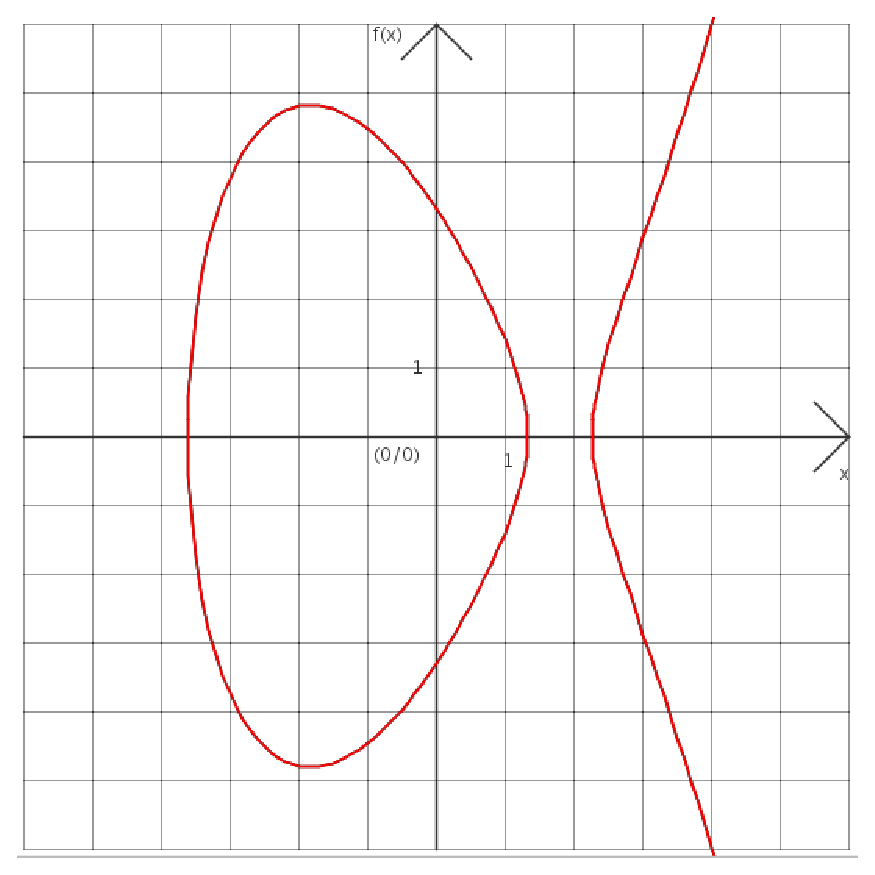
\includegraphics[width=8cm]{ec-1.eps}
\caption{Elliptische Kurve}
\end{center}
\end{figure}

Elliptische Kurven sind keine Ellipsen. Der Name kommt daher, dass die Kurven
mit den sogenannten Elliptischen Integralen zusammenhängen. 

Die wichtigste Eigenschaft von elliptischen Kurven ist, dass sie abelsche 
Gruppen bilden. Eine abelsche Gruppe ist eine Gruppe die zusätzlich zu den 
Gruppenaxiomen fordert das die Verknüpfung in der Gruppe kommutativ ist. Zur 
kurzen Wiederholung und zum Vergleich mit den Eigenschaften der Addition auf 
einer elliptischen Kurve über einem Körper sind hier die vier Gruppenaxiome
aufgelistet:
\begin{enumerate}
\item Für alle $a, b$ gilt $a\circ b\in G$. Die Verknüpfung führt nicht aus
        der Gruppe.
\item Es ist $(a\circ b)\circ c = a\circ (b\circ c)$ für alle $a,b,c\in G$. 
        Es muss das Assoziativgesetz gelten.
\item Es gibt ein Element $e\in G$, sodass $e\circ a = a\circ e = a$ für alle
        $a\in G$ gilt. Das Element $e$ heißt neutrales Element.
\item Zu jedem Element $a\in G$ gibt es ein Element $a^{-1}\in G$, sodass
        $a^{-1}\circ a= a\circ a^{-1} = e$ ist. Das Element $a^{-1}$ heißt 
        inverses Element.
\end{enumerate}

Im weiteren soll gezeigt werden welche Fälle für die Addition 
von zwei Punkten $P$ und $Q$ von $E$ unterschieden werden müssen, so dass dann
($E$,$+$) eine abelsche Gruppe bildet und wie man die scheinbar willkürliche
Definition der Addition geometrisch illustrieren kann. \\\\
Es seien $P=(x_1, y_1),\ Q=(x_2, y_2)$ zwei Punkte der elliptischen Kurve $E$.
\begin{itemize}
\item Ist $P=O$ bzw. $Q=O$, so ist $P+Q = Q$ bzw. $P+Q=P$, d.h. $O$ spielt die
        Rolle eines neutralen Elements bezüglich der Addition.

\item Liegen $P$ und $Q$ spiegelbildlich bezüglich der x-Achse, so ist $P+Q=O$.
        Insbesondere sind in diesem Fall wegen dem vorherigen Satz die Punkte 
        $P$ und $Q$ zueinander invers ($ -P=(x,-y) = Q $) .
\item Liegt weder der erste bzw. der zweite Fall vor, so ist $P+Q = R$ definiert.
        Man bestimmt den eindeutig definierten Schnittpunkt der Sekante durch 
        $P$ und $Q$ mit der Kurve und definiert $P+Q$ als seinen Spiegelpunkt
        bezüglich der x-Achse.

\end{itemize}

Die einzige Schwierigkeit um zu zeigen dass eine elliptische Kurve mit der 
Addition eine abelsche Gruppe bildet ist das Assoziativgesetz. Hierfüt gibt es 
außer dem Beweis durch Nachrechnen noch verschiedenen elegantere Beweise, etwa
mit Hilfe von doppelperiodischen Funktionen in der Funktionentheorie. Das 
neutrale Element ist per Definition $O$. 

Die Addition zweier Punkte auf einer elliptischen Kurve läßt sich auch in 
Formeln ausdrücken. Dazu sind zwei Punkte $P=(x_P, y_P)$ und $Q=(x_Q, y_Q)$ auf 
$E$ gegeben. Für die Sekante durch $P$ und $Q$ gilt 
\begin{center}
$k=\frac{y_Q-y_P}{x_Q-x_P}\ ,\ falls\ x_P \neq\ x_Q$
\end{center}
Für die Koordinaten $(x_R, y_R)$  des Punktes $P+Q = R$ ergibt sich daher nach 
einfacher Rechnung
\begin{center}
$x_R = k^2 - x_P - x_Q,\ y_R = k(x_P - x_R)-y_P$
\end{center}
Tritt hier der Fall ein das $x_P = x_Q$, aber $P\neq Q$, so gilt $P+Q=O$. Man
kann sich das so veranschaulichen das $Q$ der Spiegelpunkt von $P$ ist bezüglich
der x-Achse. Die Gerade durch $P$ und $Q$ schneidet die Kurve im unendlichen 
Punkt $O$. Das nachfolgende Schaubild veranschaulicht diesen Sachverhalt.
\begin{figure}[ht]
\begin{center}
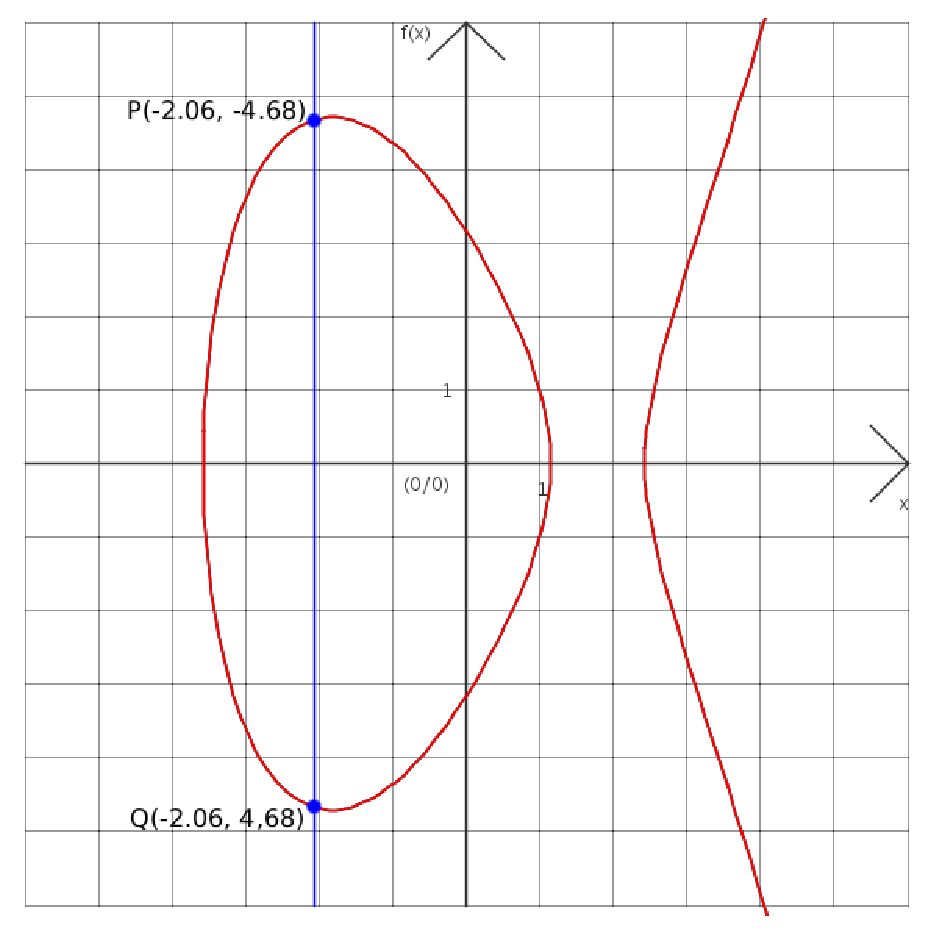
\includegraphics[width=8cm]{ec-3.eps}
\caption{Addition von $P$ und $Q$ wenn $x_P = x_Q$}
\end{center}
\end{figure}

Jetzt sei ein Punkt $P$ auf $E$ mit $y_P \neq 0$ gegeben. Dann gilt für den 
Punkt  $R=2P$
\begin{center} 
$k=\frac{3x_P^2+a}{2y_P}\ ,\ falls\ x_P = x_Q,y_P \neq 0$
\end{center}
Tritt hier der Fall $y_P = 0$ ein, so gilt $2P = O$.\\\\
{\it
\textbf{Beispiel:}\\\\
Die elliptische Kurve $E$ über $\mathbb R$ sei gegeben durch $y^2 = x^3-10x+11$.
Es sollen die beiden Punkte $P=(-3.5,1.77)$ und $Q=(0.2,3.0)$ addiert werden.\\\\ 
Mit $x_P \neq x_Q$ gilt für  
$k=\frac{y_Q-y_P}{x_Q-x_P} = \frac{3.0 - 1.77}{0.2 + 3.5} = 0.332432 $.\\\\
Für $x_R$ folgt dann $x_R = k^2-x_P-x_Q = 0.332432^2 + 3.5 - 0.2 = 3.41051$\\\\
und $y_R = k(x_P - x_R) - y_P = 0.332432(-3.5 - 3.41051) - 1.7 = -4.06728$.
}\\\\
Die Addition kann im Fall $K = \mathbb R$ durch eine geometrische Konstruktion
illustriert werden. Das folgende Schaubild zeigt die Addition von $P$ und $Q$.
Die Gerade durch $P$ und $Q$ schneidet $E$ in genau einem 
weitern Punkt $R'$. $R$ ist dann die Spiegelung dieses Punktes an der x-Achse. 
Im Fall $P=Q$ geht die Sekante in eine Tangente in $P$ über. 
\begin{figure}[ht]
\begin{center}
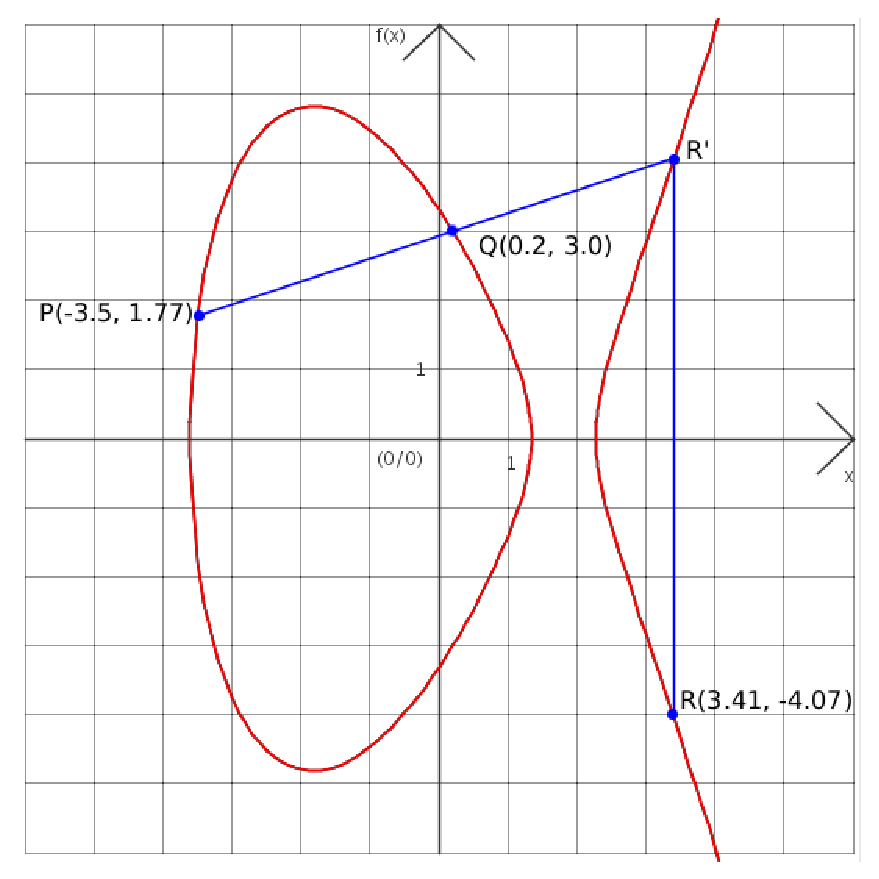
\includegraphics[width=8cm]{ec-2.eps}
\caption{Addition von P und Q auf der elliptischen Kurve E}
\end{center}
\end{figure}


Für die Gruppeneigenschaft ist die Bedingung $4a^3+27b^2 \neq 0$ notwendig. Z.B.
gilt für die Kurve $y^2-3x+2 = (x-1)^2\cdot(x+2)$ über $\mathbb R$ oder auch 
$\mathbb F_p$ mit singulärem Punkt $(1,0)$, dass $(-2,0)+(1,0) = (1,0)$. Dann
müßte aber $(-2,0)$ neutrales Element sein, was nach Vorrausetzung ein 
Widerspruch ist da unser neutrales Element $O$ ist. 

\subsubsection*{Faktorisierung mit elliptischen Kurven}
Die Frage die sich jetzt stellt ist, wie kann man elliptische Kurven zur 
Faktorisierung benützen. Zu Begin des Kapitels wurde erwähnt, dass das 
Faktorisierungsverfahren mit elliptischen Kurven stärker ist als das $(p-1)$
bzw. $(p+1)$-Verfahren, da die Anzahl der Punkte gleich der Ordnung der
elliptischen
Kurve über dem Körper $\mathbb F_p$, nicht nur von $p$ abhängt, sondern auch
von den Kurven-Parametern abhängt. Für die Anzahl der Punkte einer elliptischen 
Kurve $E$ über einem Körper $\mathbb F_p$, die mit der Gleichung $y^2 = P(x)$ 
dargestellt wird, gilt: 
\begin{center}
$Card(E) = p+1+\sum_{x=0}^{p-1}(\frac{P(x)}{p}),\ p>3$.
\end{center}
{\it
\textbf{Beispiel:}\\\\
Es wird die Primzahl $p=2803$ gewählt. Zusätzlich wählt man eine elliptische
Kurve $E$ mit der Gleichung $y^2 = x^3+x^2+b$. Der Kurvenparameter $b$ 
durchläuft die Zahlen $0-10$.\\\\
Für die Ordnungen der elliptischen Kurven $E$ über $\mathbb F_2803$ mit 
$0<=b<=10$ ergibt sich:\\

\begin{center}
\begin{tabular}{|c|c|c|}
\hline
\textbf{Kurvenparameter b} & \textbf{Ordnung} & \textbf{Primfaktorzerlegung}\\
\hline
$0$ & $2804$ & $(2,2,701)$ \\
\hline
$1$ & $2888$ & $(2,2,2,19,19)$ \\
\hline
$2$ & $2836$ & $(2,2,709)$ \\
\hline
$3$ & $2848$ & $(2,2,2,2,2,89)$ \\
\hline
$4$ & $2856$ & $(2,2,2,3,7,17)$ \\
\hline
$5$ & $2827$ & $(11,257)$ \\
\hline
$6$ & $2904$ & $(2,2,2,3,11,11)$ \\
\hline
$7$ & $2878$ & $(2,1439)$ \\
\hline
$8$ & $2819$ & $(2819)$ \\
\hline
$9$ & $2736$ & $(2,2,2,2,3,3,19)$ \\
\hline
$10$ & $2778$ & $(2,3,463)$ \\
\hline
\end{tabular}
\end{center}
Man erkennt dass je nach Wahl der Kurvenparameter die Ordnung bzw. die Anzahl
der Punkte eine elliptischen Kurve variiert.
}\\\\
Beim $(p-1)$-Verfahren hat man $k_b$ (siehe
auch den 1. Schritt des Pollard-$(p-1)$ Verfahrens) gleich dem Produkt aller
Primzahlpotenzen unterhalb einer Schranke $B$ gesetzt. Hat $n$ einen Primteiler 
$p$, so dass $(p-1)$ nur aus kleinen Primfaktoren besteht, ist
$a^{k_b} \equiv 1 mod\ p$ und falls  $a^{k_b}\not\equiv 1\ mod\ n $ ist der 
$ggT(a^{k_b}-1,n)$ ein echter Teiler von $n$. 
Das $(p-1)$ bzw. $(p+1)$-Verfahren funktioniert nur dann, wenn für eine der 
Gruppen $G(n) = \mathbb F_p^* = (\mathbb Z/p)\setminus\{0\}$, mit $p|n$, die
Ordnung aus
kleinen Primfaktoren besteht. Diese Gruppen sind aber eindeutig bestimmt durch 
$n$ und in den meisten Fällen hat keine der Gruppenordnungen die gewünschte 
Form. Bei den elliptischen Kurven kann man die Gruppenordnung $m=|E|$ also die
Anzahl der Punkte durch die Auswahl der Kurvenparameter, in dem Beispiel $b$, 
variieren und somit die Chance erhöhen, dass man ein $m$ findet das nur aus 
kleinen Primfaktoren besteht. 

Die Faktorzerlegung von $(p-1) = 2\cdot3\cdot467$ bzw. von
$(p+1) = 2\cdot2\cdot701$ enthält große Primfaktoren, d.h. sie ist ungünstig für
das $(p-1)$ bzw. das $(p+1)$-Verfahren. Schaut man sich aber die Tabelle aus 
dem vorherigen Beispiel an sieht man, dass z.B. für die Kurvenparameter 
$b=4,6,9, ...$ der elliptischen Kurve die Ordnung genau die Form hat die 
gebraucht wird.

Der Algorithmus sieht dann folgendermaßen aus. Der erste Schritt besteht aus 
der Wahl des Kurvenparameters $a$. Für den Algorithmus wird die 
elliptische Kurve $cy^2 = x^3 + ax^2 +x$ gewählt. Diese Gestalt der 
elliptischen Kurve eignet sich für Optimierungen beim berechnen des s-fachen
eines Punktes auf der Kurve. Das Polynom $x^3+ax^2+x$ hat genau dann keine
mehrfachen Nullstellen in einem Körper, wenn $a^2-4\neq 0$ ist, d.h. es gibt
keine Überkreuzungen bzw. es gibt keine singulären Punkte. 
Wie vorhin erwähnt beruht das Verfahren mit elliptischen Kurven auf der gleichen
Idee wie das  $(p-1)$-Verfahren. Deshalb werden als nächster Schritt alle
Primzahlpotenzen unterhalb einer Schranke $B$
multipliziert. Dieser Wert $s$
dient nun zur berechnung des $s$-fachen eines Punktes auf der Kurve
$E$. Ähnlich dem $(p-1)$-Verfahren bei dem durch Bildung des 
$ggT(a^{p-1}-1,n)$ der Wert von $n$ implizit auf sehr viele Primzahlen $p$
getestet wird nämlich alle, die sich durch eine beliebige Kombination der 
Primfaktoren des Exponenten $(p-1)$ von $a^{p-1}$ ergeben, wird die Berechnung
des $s$-fachen eines Punktes auf einer elliptischen Kurve $E$ über allen 
Körpern $\mathbb F_p$ durchgeführt, wobei $p$ die Primteiler von $n$ durchläuft
und so auf viele $p$ getestet wird. Doch woher weis man wann man einen Teiler 
 von $n$ gefunden hat? 

Zuerst sollte festgehalten werden das nicht direkt in 
$E(\mathbb F_p)$ gerechnet werden kann, wenn $p$ nicht bekannt ist. Deshalb kann
versucht werden, zunächst mit $\mathbb Z\ mod\ n$ zu rechnen. Im Ring 
$\mathbb Z/n$ ist das Addieren und Multiplizieren ohne weiteres erlaubt. Das 
einzige Problem besteht darin, dass in den Formeln zur berechnung von Punkten
auf $E$ durch die Nenner $(x_P-x_Q)$ bzw. $(2y_P)$ geteilt werden muss. In 
$\mathbb Z/n$ ist diese Division genau dann durchführbar wenn $(x_P-x_Q)$ bzw.
 $(2y_P)$ teilerfremd zu $n$ sind. Die Berechnung eines vielfachen bzw. 
$s$-fachen eines Punktes auf der elliptischen Kurve, scheitert genau dann
wenn diese Nenner zu $n$ nicht teilerfremd sind, d.h. es existiert ein
größter gemeinsamer Teiler! Wenn dieser ungleich $n$ ist, ist es ein nicht 
trivialer Teiler von $n$ und wenn dieser zufällig Prim ist hat man einen 
echten Teiler gefunden. In seltenen Fällen kann es vorkommen das in allen 
Körpern $\mathbb F_p$ gleichzeitig die Ausnahme auftritt. 

Tritt keine Ausnahme ein, also findet man keinen größten gemeinsamen Teiler,
wird die Schranke $B$ erhöht und wieder der $s$-fache Punkt auf der elliptischen
Kurve berechnet. Hat man die obere Grenze von $B$ erreicht, kann eine andere 
Kurve ausprobiert werden. 

Bei der Faktorisierung mit elliptischen Kurven sollte erwähnt werden, dass viele
Kurven ausprobiert werden müssen um auf einen Teiler zu kommen. Insgesamt ist
der Rechenaufwand zur Auffindung eines Primfaktors $p$ von $n$ beim Verfahren
mit elliptischen Kurven subexponentiell. 
\begin{center}
$O(exp(\sqrt{(2+o(1))\ log\ p\ log\ log\ p}))$
\end{center}
Im ungünstigsten Fall $p\approx \sqrt{n}$ ergibt sich ein Aufwand 
\begin{center}
$O(exp(\sqrt{(1+o(1))\ log\ n\ log\ log\ n}))$
\end{center}
In der Praxis können mit dem Verfahren mit elliptischen Kurven Primfaktoren von 
$n$ mit bis etwa $40$ Stellen gefunden werden. Ein großer Vorteil der elliptischen
Kurven liegt in der Möglichkeit in einem Rechnerverbund (Cluster), jedem Rechner
eine Kurve zur Berechnung zur geben. Das heißt das das Verfahren mit elliptischen
Kurven sich leicht parallelisieren läßt.

\subsubsection*{Anwendungsbeispiele:}
{\it
Die Tabelle zeigt ein paar Faktorisierungsbeispiele mit elliptischen Kurven.
Zum Vergleich wurde nur das $(p-1)$-Verfahren in Betracht gezogen um zu 
zeigen das die elliptischen Kurven eine Verbesserung gegenüber $(p-1)$ bzw.
$(p+1)$ zeigen.
}
\begin{center}
\begin{tabular}{|l|l|l|l|l|}
\hline
Nr. & Verfahren & zu faktorisierende Zahl $n$ & kleinster Primfaktor $p$ & Zeit in s\\
\hline
$1$& Elliptische Kurven & $12121212312312321312322$ & $1$ & $<1$\\
\hline
$2$&	& $576460752303423487$ & $179951$ & $2$\\
\hline
$3$&	& $23286236435849736090006331$ & $11$ & $5$\\
\hline
$4$& Pollard-$(p-1)$	& $23286236435849736090006331$ & $11$ & $18$\\
\hline
\end{tabular}
\end{center}
{\it
Man erkennt für die Zahl $3$ bzw. $4$, dass das Verfahren mit elliptischen 
Kurven die Zahl innerhalb von $5$ Sekunden faktorisiert hat, wofür das
$(p-1)$-Verfahren über $18$ Sekunden gebraucht hat. 
}



\newpage

\section{MATLAB-Integration}
\subsection{Einführung zu MEX-Dateien}
Jedes C-Programm kann aus MATLAB aufgerufen werden als wäre es
ein eingebautes Kommando. Ein C-Programm das man in MATLAB
aufrufen kann wird als MEX-Datei bezeichnet. MEX-Dateien sind
dynamisch gebundene Bibliotheken die der MATLAB-Interpreter
automatisch laden und entladen kann.

MEX-Dateien werden gebraucht wenn vorhandene C-Programme aus MATLAB
aufgerufen werden sollen ohne als M-Dateien neuimplementiert zu
werden. Werden in MATLAB-Programmen Konstrukte verwendet, z.B.
for-Schleifen, die in MATLAB nicht sehr performant sind, können sie in
C implementiert werden und die Anwendung um einiges schneller machen.

MEX-Dateien sind nicht für alle Anwendungen zu gebrauchen. Deshalb
sollte vorher überlegt werden ob überhaupt MEX-Dateien gebraucht
werden. Der größte Teil der Programmierung sollte in MATLAB erfolgen.

\subsubsection*{Ausführen von MEX-Dateien}
MEX-Dateien sind Unterprogramme die aus C-Code erstellt werden. Sie
verhalten sich wie M-Dateien und eingebaute Kommandos. MEX-Dateien
werden anhand ihrer plattformabhängigen Endung indentifiziert im
Gegensatz zu M-Dateien die eine plattformunabhängige Endung besitzen. 
Der Grund für die verschiedenen Endungen ist, dass
MEX-Dateien, die z.B. unter Windows erstellt wurden, unter Linux bzw.
irgendeinem anderen UNIX-Derivat nicht lauffähig sind. Wird unter
einer Linux-Umgebung eine MEX-Datei in MATLAB aufgerufen, weiß
MATLAB sofort dass die MEX-Datei mit der Endung \textit{mexglx}
unter Linux ausführbar ist.\\\\
Die folgende Tabelle zeigt die verschiedenen Endungen auf den
Plattformen:
\begin{center}
\begin{tabular}{|l|l|}
\hline
\textbf{Plattform} & \textbf{MEX-Datei Endung}\\
\hline
HP-UX & mexhpux\\
\hline
Linux & mexglx\\
\hline
Solaris & mexsol\\
\hline
Windows & dll\\
\hline
\end{tabular}
\end{center}
Wird z.B. die Funktion \textit{yprime} innerhalb von MATLAB aufgerufen, sucht
der Interpreter in der Liste der Verzeichnisse, die Verzeichnisse werden in
einer speziellen Umgebungsvariable gespeichert dazu später mehr, nach einer
Datei mit der plattformabhängigen Endung aus der obigen Tabelle bzw. nach einer 
Hilfe Datei die als M-File vorliegt. MEX-Dateien haben Vorrang vor M-Dateien,
d.h. gibt es zwei gleichnamige Dateien mit verschiedenen Endungen wird die
Datei mit einer MEX-Endung bevorzugt. Wenn MATLAB schließlich eine
entsprechende Datei findet wird sie geladen und ausgeführt.

\subsubsection*{MATLAB-Pfad}

Damit MATLAB die C-Funktionen ausführen kann, müssen die MEX-Dateien
(sie beinhalten die C-Funktionen) entweder in einem Verzeichnis das
MATLAB kennt oder aber im aktuellen Verzeichnis liegen. Funktionen die
im akutellen Verzeichnis liegen, haben Vorrang bzw. werden zuerst
gefunden. Das aktuelle Verzeichnis läßt sich mit dem Kommando \textit{cd}
wechseln, gleich dem \textit{cd} Shell Kommando.

Um zu erfahren welche Verzeichnisse MATLAB bekannt sind, kann man das
Kommando \textit{path} auf der Kommandozeile ausführen. Neue Verzeichnisse
lassen sich leicht mit dem \textit{addpath} Kommando hinzufügen. Eine
weitere einfache Möglichkeit stellt die GUI zur Verfügung, in dem man 
auf File->SetPath klickt. Im folgendem Dialog lässt sich über einen 
Datei-Browser das Verzeichnis hinzufügen. 	

Vorsicht geboten ist bei Dateien die auf einem Netzlaufwerk liegen. Einige
Datei-Server aktualisieren  Veränderungen nicht sofort und so kann es passieren
das MATLAB mit den alten Dateien weiterarbeitet. Abhilfe schafft der Wechsel
in ein anderes Verzeichnis und die Rückkehr ins ursprüngliche Verzeichnis.

\subsubsection*{MATLAB-Daten}
MATLAB speichert und arbeitet mit einem einzigen Daten-Objekt dem MATLAB-Array.
Alle MATLAB Variablen: Skalare, Vektoren, Matrizen, Strings, Strukturen und
Objekte werden in einem MATLAB-Array gespeichert. In C wird das MATLAB-Array als
Datentyp \textit{mxArray} deklariert. Dieser Datentyp ist mächtiger als ein
normales C-Array, denn es enthält weiterführende Informationen zum Array. Unter
anderem enthält die mxArray-Struktur Informationen über den Typ, Dimensionen, ob
das Array imaginäre Zahlen enthält usw.

Ein wichtiger Punkt beim benützen von \textit{mxArrays} ist das MATLAB
die Daten spaltenweise und nicht zeilenweise speichert, wie es in Fortran
üblich ist. Der Grund für diese Konvention ist das MATLAB ursprünglich in
Fortran geschrieben wurde.\\\\
{\it
\textbf{Beispiel:}\\\\
Gegeben sei in Array mit 3 Strings:
\begin{verbatim}
a=['house'; 'floor'; 'porch']
a =
   house
   floor
   porch
\end{verbatim}
mit den Dimensionen:
\begin{verbatim}
size(a)
ans =
     3     5
\end{verbatim}
und dem Speicherabbild:\\\\
\begin{tabular}{|l|l|l|l|l|l|l|l|l|l|l|l|l|l|l|l|}
\hline
h & f & p & o & l & o & u & o & r & s & o & c & e & r & h \\
\hline
\end{tabular}\\\\
Die Dimensionen sind nicht wie erwartet $5x3$ sondern $3x5$.
}
\subsection{Allgemeines zum Erstellen von MEX-Dateien}
Eine MATLAB Installation enthält alle Werkzeuge die notwendig
sind um mit der API zu arbeiten. Unter anderem enthält
die Installation einen C-Compiler mit dem Namen \textit{Lcc}.
Will man einen eigenen Compiler benützen muss drauf geachtet
werden das es ein ANSI C-Compiler ist und das auf
der Microsoft Plattform \textit{dll} Dateien erstellt werden können.

MATLAB unterstützt viele Compiler und liefert für den jeweiligen
Compiler eine Konfigurationsdatei mit, die die spezifischen Flags
der Compiler steuern. Auf der Homepage von MathWorks lassen sich
weitere Konfigurationsdateien runter laden und an den eigenen
Compiler anpassen. MATLAB bietet so eine bestmögliche Flexibilität
zum erstellen von MEX-Dateien.

\subsubsection*{Testen der Konfiguration}
Bevor überhaupt MEX-Dateien auf der Windows Plattform erstellt
werden können, muss die Konfigurationsdatei \textit{mexopts.bat} für den
Compiler erstellt werden. Am einfachsten ist es das mex-Skript mit
dem Aufrufparameter \textit{setup} aufzurufen.
\begin{verbatim}
mex -setup
\end{verbatim}

Mit dem mex-Skript, der Aufruf kann wahlweise vom Kommandoprompt in MATLAB
oder einer MS-DOS Eingabeaufforderung erfolgen, lassen sich jederzeit Optionen
ändern und hinzufügen. Da MATLAB einen Compiler von Haus aus mitliefert
ist es meisstens nicht nötig den Compiler zu wechseln, das mex-Skript
verwendet dann den mitgelieferten Lcc-Compiler.

Hat man sich einen eigenen Compiler konfiguriert und möchte
das eine bestimmte Konfigurationsdatei verwendet wird kann man
das mit dem \textit{-f} Parameter erzwingen.
\begin{verbatim}
mex filename -f <optionsfile>
\end{verbatim}

MATLAB liefert vorab erstellte Konfigurationsdateien für verschiedene
Compiler mit, die mit dem mex-Skript benützt werden können.

\subsection{Erstellen von C MEX-Dateien}
C MEX-Dateien werden mit dem  \textit{mex}-Skript erstellt. Das Skript
übersetzt den C-Code mit zusätzlichen API-Routinen in ein ablauffähiges
Programm.

Der Quellcode für eine MEX-Datei besteht aus zwei unterschiedlichen
Teilen. Der erste Teil ist die \textit{computational routine}. Sie
enthält den eigentlichen Anwendungscode. Der Anwendungscode kann
sowohl Berechnungen ausführen als auch Daten eingeben bzw. ausgeben.
Der zweite Teil ist die sogenannte \textit{gateway routine}. Sie
bildet die Schnittstelle zwischen MATLAB und der
\textit{computational routine}.
Die zwei Programmteile einer MEX-Datei können getrennt (in zwei Dateien)
oder zusammengefasst (in einer Datei) werden. In beiden Fällen muss
die Header-Datei \textit{mex.h} eingefügt werden. In der Header-Datei
sind die \textit{gateway routine} und die Schnittstellen-Routinen
deklariert. Der Name der \textit{gateway routine} muss auf jeden Fall
\textbf{mexFunction} lauten. Der Prototyp sieht folgendermaßen aus:
\begin{verbatim}
void mexFunction(int nlhs, mxArray *plhs[], int nrhs, const mxArray *prhs[])
\end{verbatim}
Die Parameter \textit{nlhs} und \textit{nrhs} enthalten die Anzahl
der \textit{Input} und \textit{Output} Argumente mit welchen die MEX-Datei
aufgerufen wurde. Die Parameter \textit{plhs} und \textit{prhs} sind
Vektoren die Zeiger auf die Argumente enthalten.
Alle Eingabe- und Ausgabeparameter bzw. Argumente werden in der
\textit{gateway routine} ver- und aufbereitet. Die \textit{gateway routine}
ruft die \textit{computational routine} als Unterprogramm auf.

Die übergebenen Daten, Parameter werden in der
\textit{gateway routine} in C-Datentypen \textit{umgewandelt}.
Wie vorhin erwähnt kennt MATLAB nur einen Datentyp das
\textit{mxArray}. Mit der Zeigerarithmetik in C lassen
sich darauf nicht ohne weiteres Operationen ausführen.
Will man z.B auf den ersten double-Wert aus dem
\textit{mxArray} prhs zugreifen, muss man sich zuerst
ein Pointer auf das Array holen. Das kann z.B. mit
der Funktion \textit{mexGetPr(prhs[0])} erfolgen.
Dieser Pointer kann dann wie jeder andere in der
Programmiersprache C benützt werden.

Nach dem Aufruf der \textit{computational routine} aus der
\textit{gateway routine} müssen \textit{plhs[0], plhs[1], plhs[2], ...}
auf die Daten zeigen die zurückgegeben werden sollen.
Nach erfolgreicher Abarbeitung kehrt das Programm
zurück und übergibt die Kontrolle wieder an MATLAB.\\\\
Das Übersichtsbild zeigt den generellen Ablauf bei C MEX-Dateien.\\
\begin{figure}[ht]
\begin{center}
\includegraphics[width=14cm]{matlab-mex.eps}
\caption{Übersichtsbild}
\end{center}
\end{figure}

\subsubsection*{Unterschied zwischen Funktionen mit \textit{mx} und \textit{mex}
Präfix} 
API-Funktionen mit dem Präfix \textit{mx} erlauben es \textit{mxArrays} zu
erzeugen, verändern, zerstören und darauf zu zugreifen. Ein Beispiel für so eine
Funktione wäre \textit{mxGetPi}, sie gibt einen Zeiger auf den Imaginären
Teil einer Zahl im \textit{mxArray} zurück. API-Funktionen mit dem Präfix
\textit{mex} interagieren mit der MATLAB-Umgebung.

\subsection{Praxisbeispiel}
Der folgende Abschnitt enthält Informationen und ein Besipiel,
dass zeigt wie Argumente in MEX-Dateien übergeben und
manipuliert werden können.

Die MATLAB API stellt einen kompletten Satz an Funktionen zur
Verfügung mit denen es möglich ist, die verschiedenen Datentypen
zu benützen die in MATLAB vorrätig sind. Für jeden Datentyp gibt
es einen speziellen Satz an Funktionen die für die Manipulation
des jeweiligen Datentyps verwendet werden können. Das Beispiel das
beschrieben wird zeigt auf, wie aus einer C-Datei bzw. C-Code
eine MEX-Datei entsteht.

Für das Beispiel wird eine C-Funktion verwendet die
ein Skalar quadriert. Hier der dazugehörige Code:
\begin{verbatim}
/* Datei: square.c */

#include <math.h>
void square(double y[], double x[])
{
        y[0] = x[0]*x[0];
        return;
}
\end{verbatim}

\subsubsection*{1. Schritt}
Im ersten Schritt wird die \textit{mex.h} Header-Datei eingefügt
und die \textit{gateway routine} erstellt. Wie vorhin erwähnt
muss die Gateway-Routine \textit{mexFunction} heißen und alle notwendigen
Parameter enthalten. Die Überprüfung der Argumente eines C-Programmes
wird zur Kompilierzeit vorgenommen. In MATLAB können beliebig viele
Argumente an eine MEX-Datei übergeben werden, d.h. die überprüfung der
Argumente erfolgt zur Laufzeit. Daraus folgt, dass in der
\textit{gateway routine} die Argumente geprüft und aufbereitet werden müssen.
Der folgenden Code-Abschnitt zeigt die \textit{gateway routine} in der
die richtige Anzahl und der Typ der Argumente überprüft werden und die
\textit{computational routine} welche die Berechnung durchführt. Weiterhin
werden die Rückgabewerte erzeugt und die Zeiger zugewiesen. Für weitere
Informationen siehe auch Quelltext.

\begin{verbatim}
/* Datei: mex-square.c */

#include <math.h>

/* Wichtig! Für die Erstellung der MEX-Datei */
#include <mex.h>


/* computational routine         */
/* Hier erfolgt die Berechnung   */
void square(double y[], double x[])
{
        y[0] = x[0]*x[0];
        return;
}


/* gateway routine                     */
/* Hier werden die Argumente überprüft */
/* und aufbereitet                     */ 
void mexFunction(int nlhs, mxArray *plhs[], int nrhs,
                 const mxArray *prhs[])
{
        double *x, *y;
        int mrows, ncols;

        /* Überprüfung der richtigen Anzahl von Argumenten */
        if (nrhs != 1) {
                mexErrMsgTxt("Ein Argument erforderlich!");
        } else if (nlhs > 1) {
                mexErrMsgTxt("Zu viele Rückgabewerte");
        }

        /* Das erste Argument darf nicht komplex und */
        /* muss ein double-Skalar sein               */
        mrows = mxGetM(prhs[0]);
        ncols = mxGetN(prhs[0]);
        if (!mxIsDouble(prhs[0]) || mxIsComplex(prhs[0]) ||
                !(mrows == 1 && ncols == 1)) {
                mexErrMsgTxt("Input darf nicht komplex sein");
        }

        /* Die Matrix für die Rückgabewerte erzeugen */
        plhs[0] = mxCreateDoubleMatrix(mrows,ncols, mxREAL);

        /* Zeiger den Rückgabewerten zuweisen */
        x = mxGetPr(prhs[0]);
        y = mxGetPr(plhs[0]);

        /* Die computational routine aufrufen. */
        square(y,x);
}

EOF
\end{verbatim}
\subsubsection*{2. Schritt}
Um die MEX-Datei zu erstellen wird das mex-Skript mit dem Source-Code
als Argument aufgerufen.
\begin{verbatim}
mex mex-square.c -o square       /* -o Output */
\end{verbatim}
Das Skript unternimmt alle Schritte die notwendig sind um die MEX-Datei
\textit{square} zu erstellen. Die Endung wird entsprechend der Plattform
erzeugt. MEX-Dateien lassen sich in MATLAB oder in einer Shell bzw.
Eingabeaufforderung erzeugen. Für MATLAB steht das mex.m Skript zur
Verfügung. Entsprechend der Betriebssysteme gibt es ein mex.bat und mex.sh
Skript. Egal mit welchem Skript die MEX-Datei erstellt wird, es
wird immer ein Datei \textit{square} erzeugt, welche eine plattformabängige 
Endung hat.
\subsubsection*{3. Schritt}
Nach der Erstellung lässt sich die MEX-Datei wie jede
andere M-Funktion benützen. Am MATLAB Prompt kann die
Funktion einfach aufgerufen werden, vorausgesetzt die
MEX-Datei befindet sich im aktuellen Pfad oder der Suchpfad
von MATLAB wurde um das Verzeichnis erweitert in dem sich
die MEX-Datei befindet.
\begin{verbatim}
x = 3;
y = square(x)
y =
     9
\end{verbatim}

\subsubsection*{Debugging}
Wie jede gute Programmierumgebung stellt MATLAB einen Debugger zur Verfügung.
Auf den meissten Plattformen auf denen MATLAB läuft ist es möglich MEX-Dateien,
während sie in der MATLAB-Umgebung laufen, zu debuggen. Mittlerweile ist der 
Funktionsumfang so groß, dass man jede erdenkliche Situation testen und 
überprüfen kann. Um eine MEX-Datei zu debuggen, muss dem mex-Skript der
\textit{-g} Aufrufparameter übergeben werden. 
\begin{verbatim}
mex -g filename.c
\end{verbatim}

Während dem Übersetzen entstehen zusätzliche Dateien die im selben Pfad 
liegen. Deshalb ist es nicht möglich MEX-Dateien mit Debug-Symbolen ohne
weiteres auf andere Systeme zu verteilen. Das Problem ist das jeder Compiler
spezifische Dateien erstellt, die der Entwickler meist nicht identifizieren
kann.

\section{Zusammenfassung}
Jedes Faktorisierungverfahren hat seine Vor- und Nachteile. Je nach Einsatzzweck
kommen die verschiedenen Verfahren zum Zuge. 

Bevor eines der aufwändigeren Faktorisierungsverfahren zur Anwendung kommt, wird
man die vorgegebene Zahl $n$ daraufhin untersuchen, ob sie kleine Primteiler hat.
Das beste Verfahren um  kleine Primfaktoren zu kürzen ist die Probedivision.
Meißtens werden Primzahlen bis zu einer Schranke $B$ getestet, man spricht dann
von unvollständiger Probedivision. Bei der Probedivision ergeben sich zwei
Probleme. Bei der Faktorisierung einer sehr großen Zahl müssen möglicherweise 
sehr viele Primzahlen ermittelt oder gespeichert vorliegen. Besteht die Zahl $n$
aus etwa zwei gleichgroßen Primfaktoren $s,t$ muss im schlimmsten Fall durch 
alle Primzahlen $p<s$ bzw. $p<t$ geteilt werden.
Wird versucht eine zusammengesetzte Zahl $n$ mit üblichen 150 Stellen mit der
Probedivision zu faktorisieren, bräuchte man die unglaubliche Zeit von $10^{55}$
Jahren. Ein weitere Nachteil der Probedivision ist das sie sich nicht 
parallelisieren läßt.

Das kleine Teiler einer großen Zahl mit der Probedivision gefunden werden können
ist plausibel und überrascht nicht besonders. Erstaunlich ist es aber das auch
Teiler von $n$ die nahe bei $\sqrt{n}$ liegen und daher als sehr groß eingestuft
werden leicht zu finden sind. Das Faktorisierungsverfahren von Fermat nützt
genau diese Eigenschaft. Der große Vorteil von Fermat kommt zum Vorschein 
wenn wir zwei Zahlen $p$ und $q$ haben die sich in der Nähe von $\sqrt{n}$ 
befinden. Mit einem Schlag hat man die Zahl in ihre Primfaktoren zerlegt. Man 
muß dazu sagen, hat man in den ersten Durchläufen der Suche keinen Primfaktor
gefunden kann es sein das man überhaupt keine Primfaktoren findet. Im Worst-Case
ist das Fermat-Verfahren sogar schlechter als die Probedivision. Die 
Fermat-Faktorisierung ist wie die Probedivision nicht parallelisierbar.

Das sogenannte $\rho$-Verfahren von Pollard-Brent ist bei der Auffindung
von nicht allzu grosser Faktoren recht effizient und sehr einfach. In
vielen CAS steht die Pollard-Rho-Methode an erster Stelle, wenn es darum
geht, Faktoren einer grossen Zahl zu berechnen. Der Erfolg des $\rho$-Verfahren
hängt von ein paar Faktoren ab, die mit einer guten Wahl der Startwerte, 
akzeptable Ergebnisse liefern. Ein Faktor wäre das Polynom über $\mathbb Z$. 
Das Polynom muss gute Zufallseigenschaften besitzen und darf keine maximale
Zykluslänge besitzen wie es bei Zufallszahlgeneratoren erwünscht ist. Der zweite
Faktor ist der Zufallszahlengenerator. Je genaur bzw. statistisch unabhängiger
arbeitet desto bessere Anfangwerte hat man für die Zyklen. Das $\rho$-Verfahren
ist zufallsabhängig, d.h. eine Faktorisierung kann klappen muß aber nicht. Die  
$\rho$-Methode bringt gegenüber Fermat eine Verbesserung der Laufzeit.

Beim $(p-1)$-Verfahren hofft man, dass $(p-1)$ wobei $p$ ein Primteiler von $n$
aus möglichst kleinen Primteilern zusammengesetzt ist, da es dann möglich ist, die
Zahl mit Hilfe des kleinen Satz von Fermat relativ schnell zu faktorisieren.
Vorrausgesetzt $(p-1)$ besteht aus kleinen Primzahlen, und alle diese Primzahlen
sind $B$-potenzglatt dann reicht der 1.Schritt des $(p-1)$-Verfahrens zur
Faktorisierung von $n$. Der große Vorteil gegenüber den vorherigen Verfahren ist
dass im 1. Schritt auf einen Schlag eine große Zahl von Primzahlen getestet 
werden kann. Meißtens aber kennt man den größten Primteiler von $(p-1)$ nicht 
und so weis man nicht wie groß man $B$ wählen soll. 
Das Pollard $(p-1)$-Verfahren kann keine Erfolgsgarantie geben. Ist die Schranke
$B$
in der ersten Phase zu klein findet man keinen Primfaktor der Zahl $n$. War die
1. Phase erfolgreich kann es vorkommen das in der 2. Phase kein Faktor gefunden
wurde, d.h. der Primfaktor von $n$ ist größer als die 2. Schranke. Die einzige 
Lösung ist die Schranke $B$ zu erhöhen und einen neuen Versuch zu
starten. Von der Laufzeit ist das $(p-1)$-Verfahren besser als das $\rho$-
Verfahren ist aber wie alle vorherigen von exponentieller Laufzeit.

Das Williams-$(p+1)$ ist dem $(p-1)$-Verfahren sehr ähnlich. Der 1. Schritt
ist bei beiden identisch. Der 2. Schritt der beiden unterscheiden sich, aber
man kann von der selben Laufzeit ausgehen. Deshalb wird hier nicht näher drauf
eingegangen.

Das $(p-1)$ und das $(p+1)$ Verfahren für eine große Zahl $n$ funktioniert
nur dann gut, wenn $n$ einen Primfaktor $p$ besitzt, für den $(p-1)$ und $(p+1)$
ein Produkt aus kleinen Primzahlen ist. Das Faktorisierungsverfahren mit 
elliptischen Kurven wiest diesen Nachteil nicht auf. Der Vorteil
der elliptischen Kurven gegenüber dem $(p-1)$ bzw. $(p+1)$-Verfahren ist das
durch Variationen der Kurvenparameter die Wahrscheinlichkeit erhöht werden kann,
 dass, die tatsächliche Gruppenordnung $m$ ein Produkt kleiner Primzahlen ist. 
Das hat zur Folge das eine Faktorisierung von $n$ möglich ist, obwohl für 
keinen Primfaktor $p$ von $n$ gilt, dass die Zahlen $(p-1)$ und $(p+1)$ aus 
kleinen Faktoren zusammengesetzt sind, was ja die Vorraussetzung für das 
Pollard-$(p-1)$ und Williams-$(p+1)$ Verfahren ist. Bei der Faktorisierung mit 
elliptischen Kurven kann es ein Nachteil sein, dass viele
Kurven ausprobiert werden müssen um auf einen Teiler zu kommen. 
Ein großer Vorteil der elliptischen
Kurven liegt in der Möglichkeit in einem Rechnerverbund (Cluster), jedem Rechner
eine Kurve zur Berechnung zur geben. Das heißt, dass das Verfahren mit
elliptischen Kurven sich leicht parallelisieren läßt. Die Laufzeit beim 
Verfahren mit elliptischen Kurven ist subexponentiell.


Aufbauend auf der Kettenbruchmethode von John Brillhart und Michael Morrison,
sowie inspiriert durch das lineare Sieb von Richard Schroeppel erfand Carl
Pomerance 1981 durch theoretische Überlegungen das Quadratische Sieb, welches
schneller war, als alle bis dahin bekannten Faktorisierungsverfahren.
Das quadratische Sieb ist eine Verfeinerung der Fermat-Methode und stellt einen
der am weitesten entwickelten Algorithmus zur Faktorisierung dar. Der große
Vorteil des quadratischen Siebs ist das sich die beiden Schritte: Seibschritt
und Auswahlschritt paralleisieren läßt. Es gibt einige Abwandlungen des einfachen
quadratischen Siebs, z.B. das MPQS (Multipolynomial quadratic sieve) das nicht nur
ein Polynom über $\mathbb Z$ benützt sondern viele und so die Chance erhöht
Zahlen zu finden die $B$-glatt sind. Es ist bisher nicht gelungen, die
Laufzeit des quadratischen Siebs endgültig zu bestimmen, da Annahmen über die
Verteilung der $B$-glatten Zahlen innerhalb der $f(s)$-Werte,
die zur Bestimmung der Laufzeit notwendig sind, bisher nicht
bewiesen werden konnten. Die Laufzeit gliedert sich zwischen subexponentieller
und expontieller Laufzeit ein.

Der effizienteste Faktorisierungsalgorithmus, dessen Laufzeit bewiesen
werden konnte, ist ein probabilistischer Algorithmus mit erwarteter
Laufzeit $e^{(1+o(1))(log\ n)^{\frac{1}{2}}(log\ log\ n)^{1-\frac{1}{2}}}$, mit
der gleichen Laufzeit wie das quadratische Sieb. Die Laufzeit der
elliptischen Kurven hängt nicht von dem kleinsten Primfaktor $p$ der
Zahl $n$ ab. Sollten die Primfaktoren einer Zahl $n$ relativ klein
sein, so hat diese Methode eine deutlich kürzere Laufzeit als das
quadratische Sieb, sollten beide Teiler jedoch in der Größenordnung
von $\sqrt{n}$ liegen, kann man von einer Laufzeit gleich dem
quadratischen Sieb ausgehen. Da bei auf dem Faktorisierungsproblem
basierenden Verschlüsselungsverfahren die beiden Primzahlen in
vergleichbarer Größenordnungen liegen, bringt die Elliptische Kurven
Methode keinen vorteil.

1988 wurde von Pollard das Zahlenkörpersieb entdeckt. Dies basiert auf
der algebraischen Zahlentheorie. Dabei wurde eine Möglichkeit entdeckt,
die schon aus dem quadratischen Sieb bekannte Variablen $x$ und $y$
systemtisch aus relativen kleinen Zahlen zusammenzusetzen. Der Aufwand
ist wesentlich geringer als beim quadratischen Sieb aber das Zahlenlkörpersieb
kommt wesentlich näher an einem Polynomialzeitalgorithmus heran als
andere bekannte Verfahren.

Es gab in den letzten Jahren große Fortschritte in dem Bereich der
Faktorisierung. Bisher ist noch kein Algorithmus entdeckt worden, mit
dem es möglich ist, die Faktoren einer Zahl in polynomialer Laufzeit
zu bestimmen.

Sollte so ein Algorithmus exisitieren würden Verfahren wie RSA,
SSL, GPG, PGP und alle die auf dem Faktorisierungsproblem basieren
von einem Tag auf den anderen unsicher werden.

\begin{thebibliography}{99}
\bibitem{1a} K. Reis, G. Schneider, Basiswissen Zahlentheorie
Springer-Verlag Berlin Heidelberg 2005
\bibitem{a} Remmert , Reinhold Ullrich , Peter , Elementare Zahlentheorie,
Birkhäuser
\bibitem{b} Scott Contini, Factoring Integers with the SIQS
\bibitem{c} H.-G. Gräbe, Zahlen und Primzahlen http://www.informatik.uni-leipzig.de/\~graebe
\bibitem{d} O. Forster: Algorithmische Zahlentheorie, Vieweg-Verlag 1996
\end{thebibliography}

\newpage
\section{Anhang}
\subsection{Pseudo Code}
\begin{verbatim}


(*--------------------------------------------------------*)
(*
** (p-1)-Faktorisierung mit big prime variation
*)
function p1_factbpv(N,bound1,bound2: integer): integer;
var
    base, d, ex, B0: integer;
begin
    base := 2 + random(N-2);
    write("working ");
    for B0 := 0 to bound1-1 by 256 do
        ex := ppexpo(B0,min(B0+256,bound1));
        base := base**ex mod N;
        d := gcd(base-1,N); write('.');
        if d > 1 then return d; end;
    end;
    if d = 1 then
        writeln(); write("entering big prime variation ");
        d := bigprimevar(base,N,bound2);
    end;
    return d;
end;
(*-----------------------------------------------------*)
(*
** Hilfsfunktion fuer p1_factbpv
** Setzt die Existenz einer Datei "primdiff.dat"
** mit den halben Differenzen aufeinander folgender
** ungerader Primzahlen bis 10**6 voraus, die durch
** den Aufruf primdiff(10**6) erzeugt wird.
*)
function bigprimevar(y,N,bound: integer): integer;
const
    DiffFile = "primdiff.dat";
    maxhdiff = 57;
var
    X: array[maxhdiff+1];
    f: file;
    i, k, y2, q, q0, d, z, count: integer;
begin
    X[0] := 1; y2 := y*y mod N;
    for i := 1 to maxhdiff do X[i] := X[i-1]*y2 mod N; end;
    bound := min(bound,10**6);
    if not open_read(f,DiffFile,binary) then
        writeln("unable to open file ",DiffFile); halt(0);
    end;
    q := 3; y := y**q mod N; z := y-1;
    d := 0; count := 1;
    while q < bound do
        k := read_byte(f); q := q + 2*k;
        y := y*X[k] mod N;
        z := z*(y-1) mod N;
        if inc(count) >= 1000 then
            write('.'); count := 0;
            d := gcd(z,N);
            if d > 1 then break; end;
        end;
    end;
    close(f);
    return d;
end;
(*-----------------------------------------------------*)


(************************************************************)
(*
** Otto Forster: Algorithmische Zahlentheorie
** Vieweg-Verlag 1996, ISBN 3-528-06580-X
**
** ARIBAS-Code zu Paragraph 18
** Die (p+1)-Faktorisierungs-Methode
*)
(*--------------------------------------------------------------*)
function pp1_factorize(N,bound: integer): integer;
const
    anz0 = 128;
var
    a, d, n, B0, B1, ex: integer;
begin
    a := 2 + random(N-3);
    if (d := gcd(a*a-1,N)) > 1 then return d end;
    write("working ");
    for B0 := 0 to bound-1 by anz0 do
        B1 := min(B0+anz0, bound);
        ex := ppexpo(B0,B1);
        a := mod_coshmult(a,ex,N);
        if a = 1 then return 0 end;
        write('.');
        d := gcd(a-1,N);
        if d > 1 then
            writeln();
            writeln("factor found with bound ",B1);
            return d;
        end;
    end;
    return 0;
end;
(*--------------------------------------------------------------*)
function ppexpo(B0,B1: integer): integer;
var
    x, m0, m1, i: integer;
begin
    x := 1;
    m0 := max(2,isqrt(B0)+1); m1 := isqrt(B1);
    for i := m0 to m1 do
        x := x*i;
    end;
    if odd(B0) then inc(B0) end;
    for i := B0+1 to B1 by 2 do
        if prime32test(i) > 0 then x := x*i end;
    end;
    return x;
end;
(*--------------------------------------------------------------*)



(*----------------------------------------------------------------*)
(*
** Implementierung des Pollardschen Rho-Verfahrens zur Faktorisierung
** Bemerkung: In ARIBAS als eingebaute Funktion mit dem Namen
** rho_factorize vorhanden
*)
(*----------------------------------------------------------------*)
(*
** Versucht, die Zahl N zu faktorisieren. Der Parameter anz
** ist eine Schranke fuer die Anzahl der Iterationen.
** Ein Faktor p von N wird im allgemeinen gefunden, falls
** anz groesser als die Quadratwurzel von p ist.
*)
function poll_rho(N,anz: integer): integer;
const
    anz0 = 256;
var
    x, y, i, d, P: integer;
begin
    y := x := random(N);
    write("working ");
    for i := 0 to (anz-1) div anz0 do
        P := accumdiff(x,y,N,anz0);
        write('.');
        d := gcd(P,N);
        if d > 1 and d < N then
            writeln(); writeln("factor found after ");
            writeln((i+1)*anz0," iterations");
            return(d);
        end;
    end;
    return 0;
end;
(*----------------------------------------------------------------*)
function accumdiff(var x,y: integer; N, anz: integer): integer;
var
    i, P: integer;
begin
    P := 1;
    for i := 1 to anz do
        x := (x*x + 2) mod N;
        y := (y*y + 2) mod N;
        y := (y*y + 2) mod N;
        P := P * (y-x) mod N;
    end;
    return P;
end;




(*-----------------------------------------------------------------*)
(*
** Zugrunde liegt eine elliptische Kurve c*Y*Y = X*X*X + X + b
** Gerechnet wird simultan ueber allen Koerpern Fp, wobei
** p ein Teiler von N ist.
** Es wird vorausgesetzt, dass gcd(N,6) = 1.
** Das Argument x ist die x-Koordinate eines Punktes Q = (x,y)
** auf der elliptischen Kurve.
** Es wird die x-Koordinate des Punktes S := s*Q berechnet.
** Falls waehrend der Berechnung ein Nenner auftaucht, der
** nicht zu N teilerfremd ist, wird das Paar (d, 0) zurueckgegeben,
** wobei d der gemeinsame Teiler des Nenners mit N ist.
** Sonst wird das Paar (xS, 1) zurueckgegeben, wobei xS die
** x-Koordinate des Punktes S ist.
**
** Diese Funktion ist analog zur eingebauten ARIBAS-Funktion
**      mod_pemult(x,s,a,N: integer): array[2];
** die dasselbe fuer die Kurve c*Y*Y = X*X*X + a*X*X + X durchfuehrt.
*)
(*-----------------------------------------------------------------*)
function ellmult(x,s,b,N: integer): array[2];
var
    x1,xold,z,zinv,P1,P1inv,Pprime,mu,k: integer;
begin
    if s = 0 then return (0,0); end;
    x1 := x; z := 1;
    P1 := (x*x*x + x + b) mod N;
    P1inv := mod_inverse(P1,N);
    if P1inv = 0 then return (gcd(N,P1),0); end;
    for k := bit_length(s)-2 to 0 by -1 do
        zinv := mod_inverse(2*z,N);
        if zinv = 0 then return (gcd(N,2*z),0); end;
        Pprime := (3*x*x + 1) mod N;
        mu := (Pprime * P1inv * zinv) mod N;
        xold := x;
        x := (P1*mu*mu - 2*xold) mod N;
        z := (-z - mu*(x - xold)) mod N;
        if bit_test(s,k) then
            mu := mod_inverse(x-x1,N);
            if mu = 0 then return (gcd(N,x-x1),0); end;
            mu := mu*(z-1) mod N;
            x := (P1*mu*mu - x - x1) mod N;
            z := (-1 - mu*(x - x1)) mod N;
        end;
    end;
    return (x,1);
end;
(*--------------------------------------------------------*)
function ec_factorize(N, bound, anz: integer): integer;
var
    k, a, d: integer;
begin
    write("working ");
    for k := 1 to anz do
        a := random(64000);
        d := gcd(a*a-4,N);
        if d = 1 then
            write('.');
            d := ec_fact0(N,a,bound);
        end;
        if d > 1 and d < N then return d; end;
    end;
    return 0;
end;
(*--------------------------------------------------------*)
function ec_fact0(N,a,bound: integer): integer;
const
    anz0 = 128;
var
    x, B0, B1, s, d: integer;
    xx: array[2];
begin
    x := random(N);
    for B0 := 0 to bound-1 by anz0 do
        B1 := min(B0+anz0,bound);
        s := ppexpo(B0,B1);
        xx := mod_pemult(x,s,a,N);
        if xx[1] = 0 then
            d := xx[0];
            if d > 1 and d < N then
                writeln(); write("factor found with curve ");
                writeln("parameter ",a," and bound ",B1);
            end;
            return d;
        else
            x := xx[0];
        end;
    end;
    return 0;
end;
\end{verbatim}
\end{document}
